\documentclass[12pt,fleqn,a4paper,oneside]{mybook} %Final!!!
%\documentclass[11pt,fleqn,a4paper,draft]{mybook} %DRAFT - highlights overflow, leaves out images

%\usepackage{microtype}
\usepackage[slovak]{babel}
\usepackage[utf8]{inputenc}
\usepackage[T1]{fontenc}
\usepackage[normalem]{ulem}
\usepackage{mathtools}  					
\usepackage{graphicx}
%\usepackage{subfig}
\usepackage{subfigure}
\usepackage{enumerate}
\usepackage{etoolbox}                       %Problematic URL in reference
\apptocmd{\sloppy}{\hbadness 10000\relax}{}{}%Removes badness warnings
%This is to remove warnings resulting by otherwise OK URL's
\usepackage[hyphens]{url}
\usepackage{notes}
\usepackage{indentfirst}
%\usepackage[demo]{graphicx}
\usepackage{upgreek}
\usepackage{multicol}
%This custom command defines how the literal menus look like.
\newcommand{\gui}[1]{{\emph{#1}}} %Gui commands, icon names, buttons
 % All code, functions, variables are typed like this
\newcommand{\code}[1]{{\lstinline[columns=fixed]{#1}}}

\newcommand{\angl}[1]{{\footnote{\emph{angl.}\ {#1}}}} %Shorthand english equivalent


\usepackage[left=25mm,right=25mm,top=25mm,bottom=25mm,paperwidth=210mm,paperheight=297mm,includehead]{geometry}

\usepackage{titlesec}
\titleformat{\chapter}[hang]{\normalfont\huge\bfseries}{\thechapter}{1em}{}



\DeclarePairedDelimiter{\diagpars}{(}{)}
\newcommand{\diag}{\operatorname{diag}\diagpars}

\let\oldhat\hat
\renewcommand{\vec}[1]{\boldsymbol{\mathbf{#1}}}
%\renewcommand{\hat}[1]{\oldhat{\boldsymbol{\mathbf{#1}}}}


\usepackage{amsthm}
\usepackage{etoolbox}% http://ctan.org/pkg/etoolbo
\theoremstyle{definition}
\newtheorem{exmp}{Pr\'{i}klad}[chapter]
\AtEndEnvironment{exmp}{\null\hfill\qedsymbol}

\usepackage{listings,color} 			    %To list Matlab code
\definecolor{mygrey}{gray}{0.5}	        %Define a gray color
\lstset{
basicstyle=\ttfamily,
numbers=none,
commentstyle=\color{mygrey},
breaklines=true,
}
%extended Matlab language
\lstdefinelanguage{exMatlab}[]{Matlab}      %Defining expanded Matlab
{morekeywords={rng,pyulear,plot,hold,randn,filter,length,abs,periodogram,fft,sin,randn,xcorr,fminsearch,dlqr,predmodelqp,dlyap,ones,linprog,quadprog,optimset,qpOASES,qpOASES_sequence,sysStruct,probStruct,mpt_control,volume,hull,extreme,mpt_exportc,mpt_getInput,sdpvar,blkdiag,sdpsettings,solvesdp,geomean,double},
sensitive=true,
alsoletter={_}
}

\usepackage{xcolor}
\lstset { %
	language=C++,
	backgroundcolor=\color{white}, % set backgroundcolor
	basicstyle=\footnotesize,% basic font setting
}


\pagestyle{empty}

\begin{document}
%%%%%%% Zaciaatok %%%%%%%%

\renewcommand\thepage{\roman{page}}
\pagenumbering{roman}
\thispagestyle{empty}

\noindent \begin{center}
\textbf{{\large{}SLOVENSKÁ TECHNICKÁ UNIVERZITA V BRATISLAVE}}\\
\textbf{{\large{}STROJNÍCKA FAKULTA}}\textbf{\large{} }\\
\vspace{3cm}
\par\end{center}

\noindent \begin{center}
\vspace{3cm}
\par\end{center}



\begin{center}
\textbf{\textsc{\Large{}AeroShield: Miniatúrny experimentálny modul aerokyvadla}}\\
\par\end{center}{\Large \par}

\begin{center}
\textbf{\large{}Bakalárska práca}\\
\par\end{center}{\large \par}

\begin{center}
{\large{}SjF-číslo b. práce}\\
\par\end{center}{\large \par}



\vfill
\noindent \textbf{\large{}2022} \hfill \textbf{\large{}Bc. Peter Tibenský}
\cleardoublepage

\thispagestyle{empty}

\noindent \begin{center}
\textbf{{\large{}SLOVENSKÁ TECHNICKÁ UNIVERZITA V BRATISLAVE}}\\
\textbf{{\large{}STROJNÍCKA FAKULTA}}\textbf{\large{} }\\
\vspace{3cm}
\par\end{center}

\noindent \begin{center}
\vspace{3cm}
\par\end{center}



\begin{center}
\textbf{\textsc{\Large{}AeroShield: Miniatúrny experimentálny modul aerokyvadla}}\\
\par\end{center}{\Large \par}

\begin{center}
\textbf{\large{}Bakalárska práca}\\
\par\end{center}{\large \par}

\begin{center}
{\large{}SjF-12345-67890}\\
\end{center}


\vfill
\begin{flushleft}
$\begin{array}{ll}
\text{Študijný odbor:}&\text{Automatizácia a informatizácia strojov a procesov}\\
\text{Študijný program:}&\text{5.2.14 automatizácia}\\
\text{Školiace pracovisko:}&\text{Ústav automatizácie, merania a aplikovanej informatiky}\\
\text{Vedúci záverečnej práce:}&\text{Ing. Mgr. Anna Vargová.}\\
\text{Konzultant:}&\text{Ing. Erik Mikuláš}\\
\end{array}$
\end{flushleft}
\vspace{0.5cm}
\noindent \textbf{\large{}Bratislava, 2022} \hfill \textbf{\large{}Peter Tibenský}
\cleardoublepage

\frontmatter
Úlohou študenta je navrhnúť, realizovať a sériovo vyrobiť rozširovací modul pre prototypizačnú platformu Arduino v rámci open-source projektu „AutomationShield“. Jedná sa o návrh miniaturizovaného laboratórneho experimentu so spätnoväzobným riadením tzv. aerokyvadla, spolu s ovládacím softvérom a inštruktážnymi príkladmi. Študent navrhne plošný spoj v CAD prostredí DipTrace, vytvorí programátorské rozhranie (API) v jazyku C/C++ pre Arduino IDE, ďalej pre MATLAB a Simulink. Študent manažuje verzie projektu v Git pre GitHub a píše úplnú dokumentáciu v MarkDown.

\cleardoublepage

	

\null
\vfill
\noindent
\section*{Čestné prehlásenie}

Vyhlasujem, že predloženú záverečnú prácu som vypracoval samostatne pod vedením vedúceho záverečnej práce, s použitím odbornej literatúry a ďalších informačných zdrojov, ktoré sú citované v práci a uvedené v zozname použitej literatúry. Ako autor záverečnej práce ďalej prehlasujem, že som v súvislosti s jej vytvorením neporušil autorské práva tretích osôb.\\

\noindent Bratislava, 23. máj 2022 \hfill $\begin{array}{rl}
                                          &\text{..................................}\\
                                          &\text{Vlastnoručný podpis}\\
                                           \end{array}$
\cleardoublepage


	

\null
\vfill
\noindent

V prvom rade by som rád poďakoval vedúcej mojej bakalárskej práce, Ing. Mgr. Anne Vargovej, za odbornú pomoc,ľudský prístup a cenné rady pri vypracovávaní práce. Ďalej chcem poďakovať aj konzultantovi bakalárskej práce, Ing. Erikovi Mikulášovi, za pomoc a pripomienky pri tvorbe dosky plošných spojov a návrhu 3D modelov.\\

\noindent Bratislava, 20. mája 2018 \hfill  Peter Tibenský
\cleardoublepage


	


\noindent
\textbf{Názov práce:} AeroShield: Miniatúrny experimentálny modul aerokyvadla\\
\textbf{Kľúčové slová: } Arduino, AutomationShield, PID, AeroShield, AeroPendulum \\
\textbf{Abstrakt: } Cieľom bakalárskej práce je návrh experimentálneho modulu pre platformu Arduino. Tento modul má podobu externého shieldu, ktorý sa dá jednoducho pripojiť ku doskám Arduino a slúži na výučbu základov riadenia. Ich súčasťou je hardwareova a softwaerova časť. V rámci bakalárskej práce bol navrhnutý jeden modul s názvom AeorShield.   \\

\noindent
\textbf{Title:}AeroShield: Miniature experimental module of aeropendulum \\
\textbf{Keywords: }  Arduino, AutomationShield, PID, AeroShield, AeroPendulum\\
\textbf{Abstract: } The aim of the bachelor's thesis is to design an experimental module for the Arduino platform. This module takes the form of an external shield that can be easily connected to Arduino boards and is used to teach the basics of control. Each module consist of hardware and a software part. As a part of this bachelor thesis, one module was designed, the AeroShield.
\cleardoublepage

%%%%%% \chapter*{Predhovor}
\thispagestyle{empty}

Myslel som si že ma táto téma bude baviť. Až pokial som si neuvedomil, že to nebude až také jednoduché... 

Už od malička ma fascinovala elektronika a všetko čo sa vedelo pohybovať a ja som to vedel riadiť. Volba tejto bakalárskej práce preto bola jasnou voľbou. 

\cleardoublepage

 %%%%%%
\tableofcontents
\thispagestyle{empty}
\cleardoublepage
\listoffigures
%%%%%% Jednotlive kapitoly %%%%%%%%%
\pagestyle{plain}
\pagenumbering{arabic}
\setcounter{page}{1}

\mainmatter
\chapter*{Úvod}
\label{UVOD}
\addcontentsline{toc}{chapter}{Úvod}

%V úvode autor podrobnejšie ako v predhovore, pritom výstižne a krátko charakterizuje stav poznania alebo praxe v špecifickej oblasti, %ktorá je predmetom záverečnej práce. Autor presnejšie ako v predhovore vysvetlí ciele práce, jej zameranie, použité metódy a stručne %objasní vzťah práce k iným prácam podobného zamerania. V úvode netreba zachádzať hlbšie do teórie. Netreba podrobne opisovať metódy, %experimentálne výsledky, ani opakovať závery prípadne odporúčania.
%Úvod začína na novej  strane.


Cieľom tejto bakalárskej práce je návrh, výroba a naprogramovanie modernej učebnej pomôcky AeroShieldu (ďalej len „shield”), ktorý slúži na výuku základov teórie riadenia a elektrotechniky.

Učebné pomôcky sú nevyhnutnou, no často zanedbávanou súčasťou výuky. Študenti si vďaka nim môžu lepšie predstaviť a pochopiť problematiku daného učiva, keďže môže pracovať nie len s počítačovými modelmi sústavy, ale aj s jej fyzickou reprezentáciou. 
Avšak, takéto pomôcky bývajú častokrát príliš zložité na používanie a drahé \cite{Hor}. Z toho dôvodu, je ich použitie pri výučbe nepraktické.

Za cieľom sprístupnenia experimentálnych modulov širokej verejnosti bol založený projekt AutomationShield, ktorý ponúka pomerne jednoduché a cenovo dostupné experimentálne moduly ako open-source\footnote[1]{Open-source je zo všeobecného pohľadu akákoľvek informácia ktorá je dostupná verejnosti bez poplatku(s voľným prístupom), s ohľadom na fakt, že jej voľné šírenie zostane zachované.} študentské projekty.

Vhodnou platformou na implementáciu týchto modulov sú napríklad prototypizačné dosky Arduino ktoré sú taktiež open-source. Ich nízka cena a celosvetová popularita, spojená s obrovským množstvom návodov, informácii a pomôcok, vytvára ideálnu platformu pre začínajúcich, ako aj pokročilých, programátorov, elektrotechnikov alebo hobby nadšencov.

V bakalárskej práci je opísaný postup výroby a fungovania shieldu s dôrazom na zrozumiteľnosť jednotlivých aspektov aj čitateľom, ktorý o danej téme nie sú dokonale oboznámený. Na začiatku bakalárskej práce, v časti hardware, je opísaný základný princíp fungovania shieldu a následne jeho jednotlivé súčiastky. Pochopenie fungovania jednotlivých súčiastok shieldu je kritické pre správnu manipuláciu užívateľa s jeho jednotlivými časťami. Poslednú časť tvorí tvorba dosky plošných spojov pre shield v programe DipTrace.

V softvérovej časti sú bližšie predstavené jednotlivé charakteristické funkcie shieldu. Funkcie sú usporiadané do logických celkov pre ľahšiu prácu užívateľa s kódom.


\chapter{Motivácia}

Cieľom tejto bakalárskej práce je návrh učebnej pomôcky AeroShield, vo svete známej pod názvom Aeropendulum, čo v doslovnom preklade znamená vzdušné kyvadlo. Jedná sa o pomerne jednoduché zariadenie pozostávajúce z niekoľkých častí. Akčným členom tohoto zariadena je  motorček na jednosmerný prúd, ktorý má na rotor pripojené lopatky ktoré vďaka otáčaniu produkujú ťah. Motorček je zvyčajne upevnený na koniec ľahkej tyčku ktorá je v mieste otáčania pripevnená k zariadeniu na meranie uhlu pootočenia tyčky. Zariadenie na meranie pootočenia môže byť potenciometer, senzor hall efektu alebo iné \cite{senzor}. V našom prípade budeme používať senzor hall efektu ktorého fungovanie je opísané v časti hardware. Zariadenie na meranie uhlu je následne upevnené na podstavec aby sa motor mohol voľne pohybovať. Zostavenie takéhoto kyvadlo bolo cieľom tejto bakalárskej práce a jeho podobu môžete vidieť na obr. \ref{OBRAZOK 1.1}

\begin{figure}[!tbh]
\centering
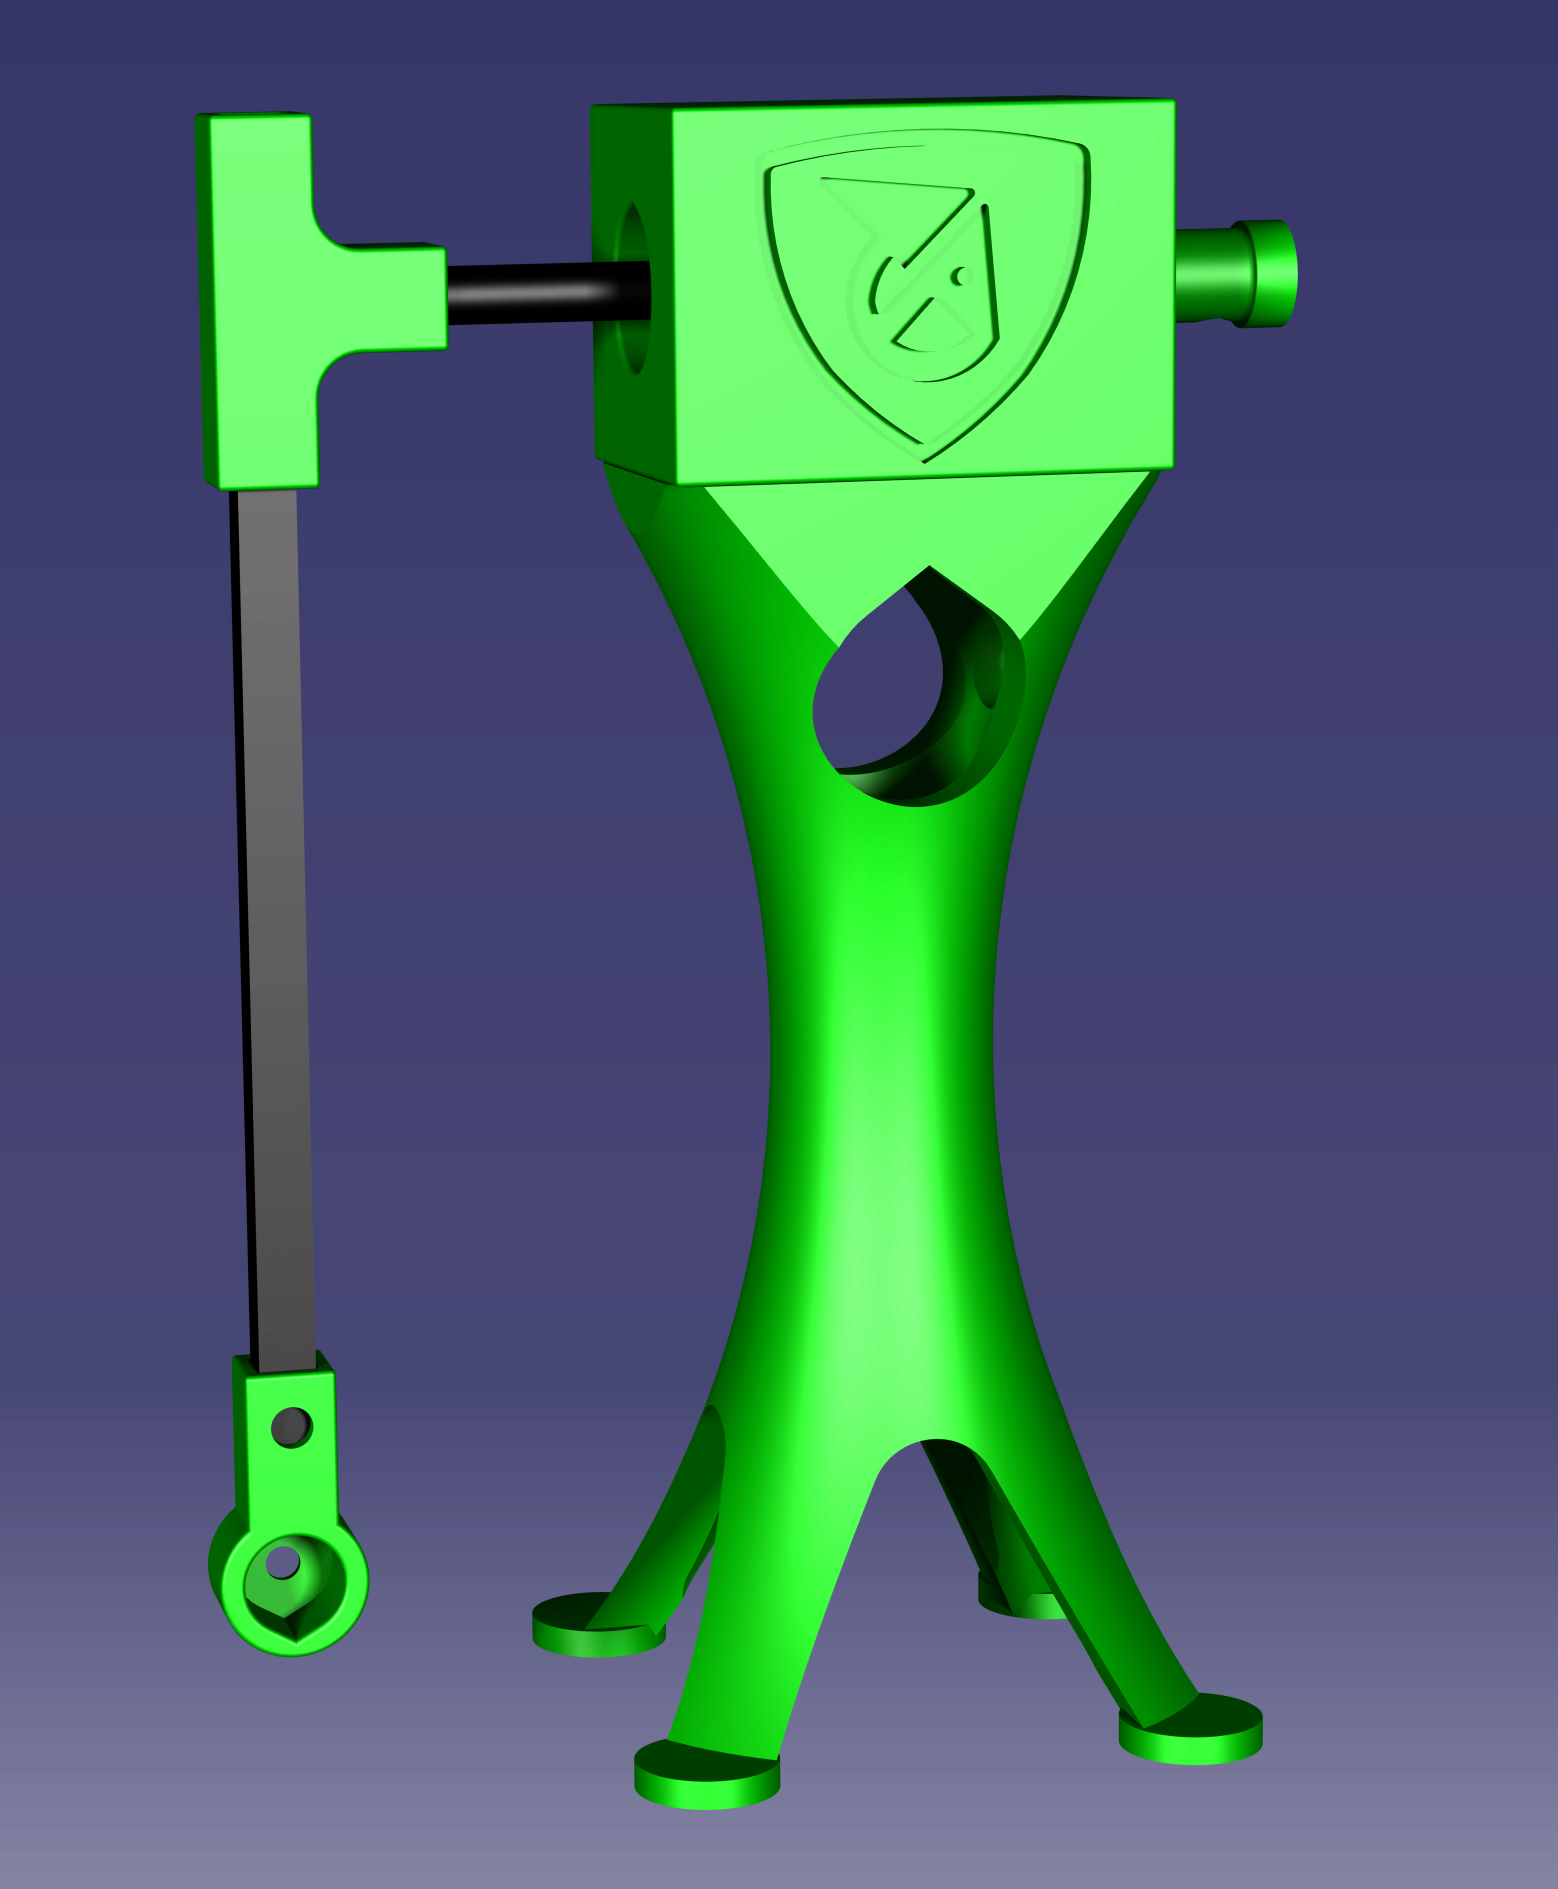
\includegraphics[width=80mm]{obr/pendulum.png}
\caption{dočasný obrázok pokial nebude hotovec final.}\label{OBRAZOK 1.1}
\end{figure}

Open-source projekt AutomationShield vyvíjaný na ústave Automatizácie, merania a aplikovanej informatiky SJF STU, je zameraný na vývoj hardwarových a softwarových nástrojov určených na vzdelávanie a doplnenie vzdelávacieho procesu. Jadrom celého projektu je tvorba rozširujúcich dosiek(shieldov) vyvíjaných pre populárny typ prototypizačných dosiek s mikrokontrolérmi Arduino, ktoré majú za ciel lepšiu výučbu strojného inžinierstva, mechatroniky a riadenia \cite{Auto}.

Zdrojový kód k AeroShieldu, ako aj ku všetkým modulom AutomationShield, nájdeme na platforme GitHub \cite{Git}, ktorá slúži ako obrovská knižnica kódov, návodov a postupov pre kohokoľvek. Na samostatnej stránke AutomationShield nájdeme zoznam jednotlivých shieldov a to v akom procese výroby sa nachádzajú. Ku každému shieldu nájdeme jeho podrobnú dokumentáciu, knižnice, zdrojové kódy ako aj predprogramované ukážky fungovania. Tým že GitHub je open-source platforma, dokumenty na stránke môže ktokoľvek upravovať alebo vylepšovať čo tvorí ideálny priestor pre rozvoj myšlienok a tvorivý proces. Na dokumentoch môže naraz pracovať niekoľko desiatok ludí, čím sa častokrát mnohonásobne urýchluje proces tvorby a hľadania chýb.

Ako už bolo spomenuté, hlavnou motiváciou tohoto projektu je nízka dostupnosť a vysoká cena podobných učebných pomôcok. Výučba je preto častokrát až príliš zameraná na memorovanie faktov a teórie, namiesto praktických experimentov a skúseností typu pokus-omyl. Jediný podobný dostupný produkt na kúpu nie ako kit, je Aeropendulum od neznámej perzskej značky Real Sim ktoré je na obr. \ref{OBRAZOK 1.2}. Študenti si omnoho rýchlejšie osvoja metódy programovania a automatizácie, pokiaľ majú možnosť experimenty sami tvoriť a skúmať vplyv reálnych výstupov na zvolené vstupy. S úmyslom priniesť širokej verejnosti lacnejšiu a výkonnejšiu alternatívu vtedajším mnohonásobne drahším a menej výkonným prototypizačným doskám \cite{stamp}, prišla na trh v roku 2005 prototypizačná doska Arduino. Projekt vznikol v Taliansku ako kolaborácia medzi viacerými nadšencami elektrotechniky a programovania, na ktorých čele bol Massimo Banzi.

\begin{figure}[!tbh]
\centering
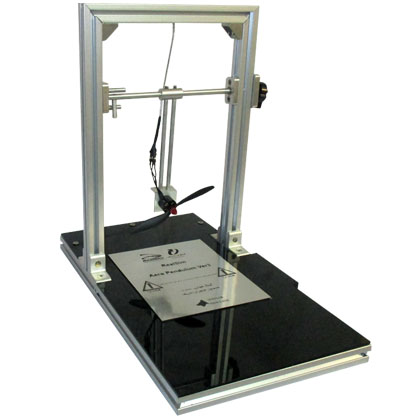
\includegraphics[width=80mm]{obr/pendulum.jpg}
\caption{Aeropendulum značky Real Sim.}\label{OBRAZOK 1.2}
\end{figure}

Veľkou výhodou dosiek Arduino a ich nadstavbových shieldov je fakt, že sú pomerne lacné a majú malé rozmery (Arduino UNO: 68.6*53.4mm \cite{UNO} ). Tieto fakty umožňujú študentom pracovať na experimentoch nielen na pôde školy, ale experimenty si môžu zobrať domov a pracovať na nich aj mimo vyučovacieho procesu. Na správne fungovanie a programovanie dosky nám postačuje len USB kábel a samotná doska. Vzhľadom na nízky počet potrebných súčiastok a fakt, že mikročip arduina je v prípade poruchy jednoducho vymenitelný \footnote[2]{Tento fakt platí pri mikročipoch typu DIP(Dual in-line package) ktoré stačí jednoducho vytiahnúť z konektora bez použitia spájkovania.}, je ich používanie na školách príjemné a jednoduché. Pre naše účely je vhodná doska Arduino UNO ktorú môžeme vidieť na obr. \ref{OBRAZOK 1.3}. Na doske sa nachádza 14 digitálnych a 6 analógových pinov. Niektoré piny sú označené špeciálnym symbolom ~, tieto piny sú schopné produkovať PWM\footnote[3]{Šírková modulácia impulzov alebo PWM je technika na dosiahnutie analógových výsledkov pomocou digitálnych prostriedkov a to, za pomoci striedania dĺžok medzi High a Low stavom resp. zapnutý a vypnutý stav.} signál ktorý potrebujeme na správne ovládanie motoru kyvadla.

\begin{figure}[!tbh]
\centering
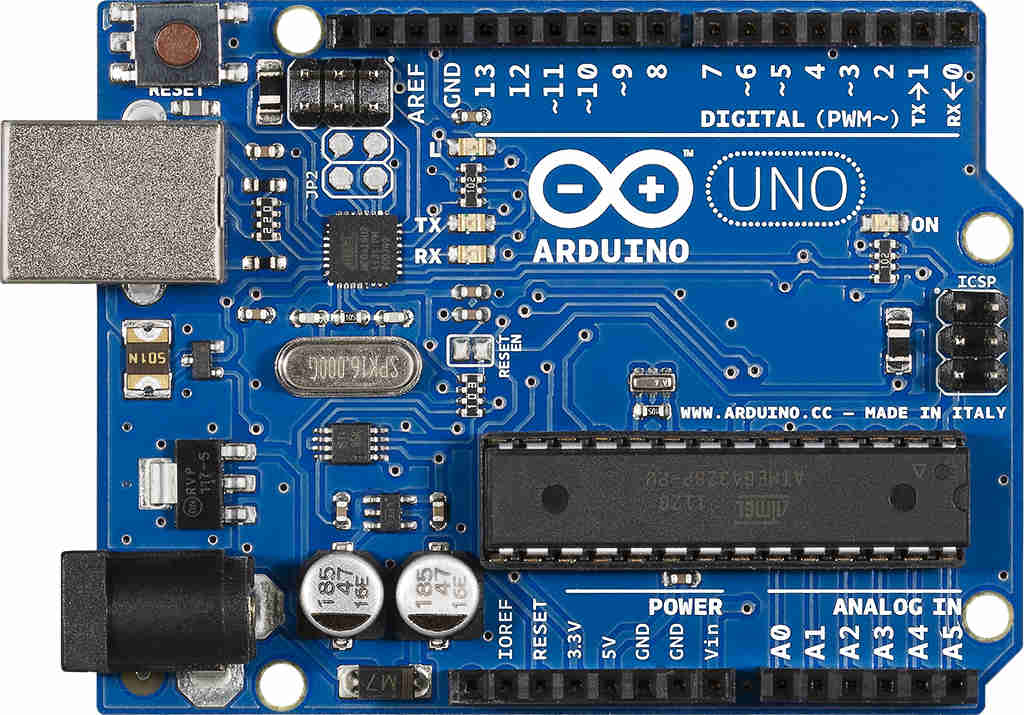
\includegraphics[width=80mm]{obr/arduino.jpg}
\caption{Arduino UNO.}\label{OBRAZOK 1.3}
\end{figure}




\chapter{AeroShield}

Téma tejto bakalárskej práce vznikla ako pokračovanie, na už započatom projekte aero kyvadla. Prvá verzia dosky a samotného kyvadla vznikla ako záverečný projekt na predmet Mikroprocesorová technika. Na projekte pracovala pätica študentov: . Schému zapojenia hlavnej dosky, ako aj fotografiu napájkovanej verzie môžeme vidieť na obr.\ref{OBRAZOK 2.1.1}.


\begin{figure}[!tbh]
\centering
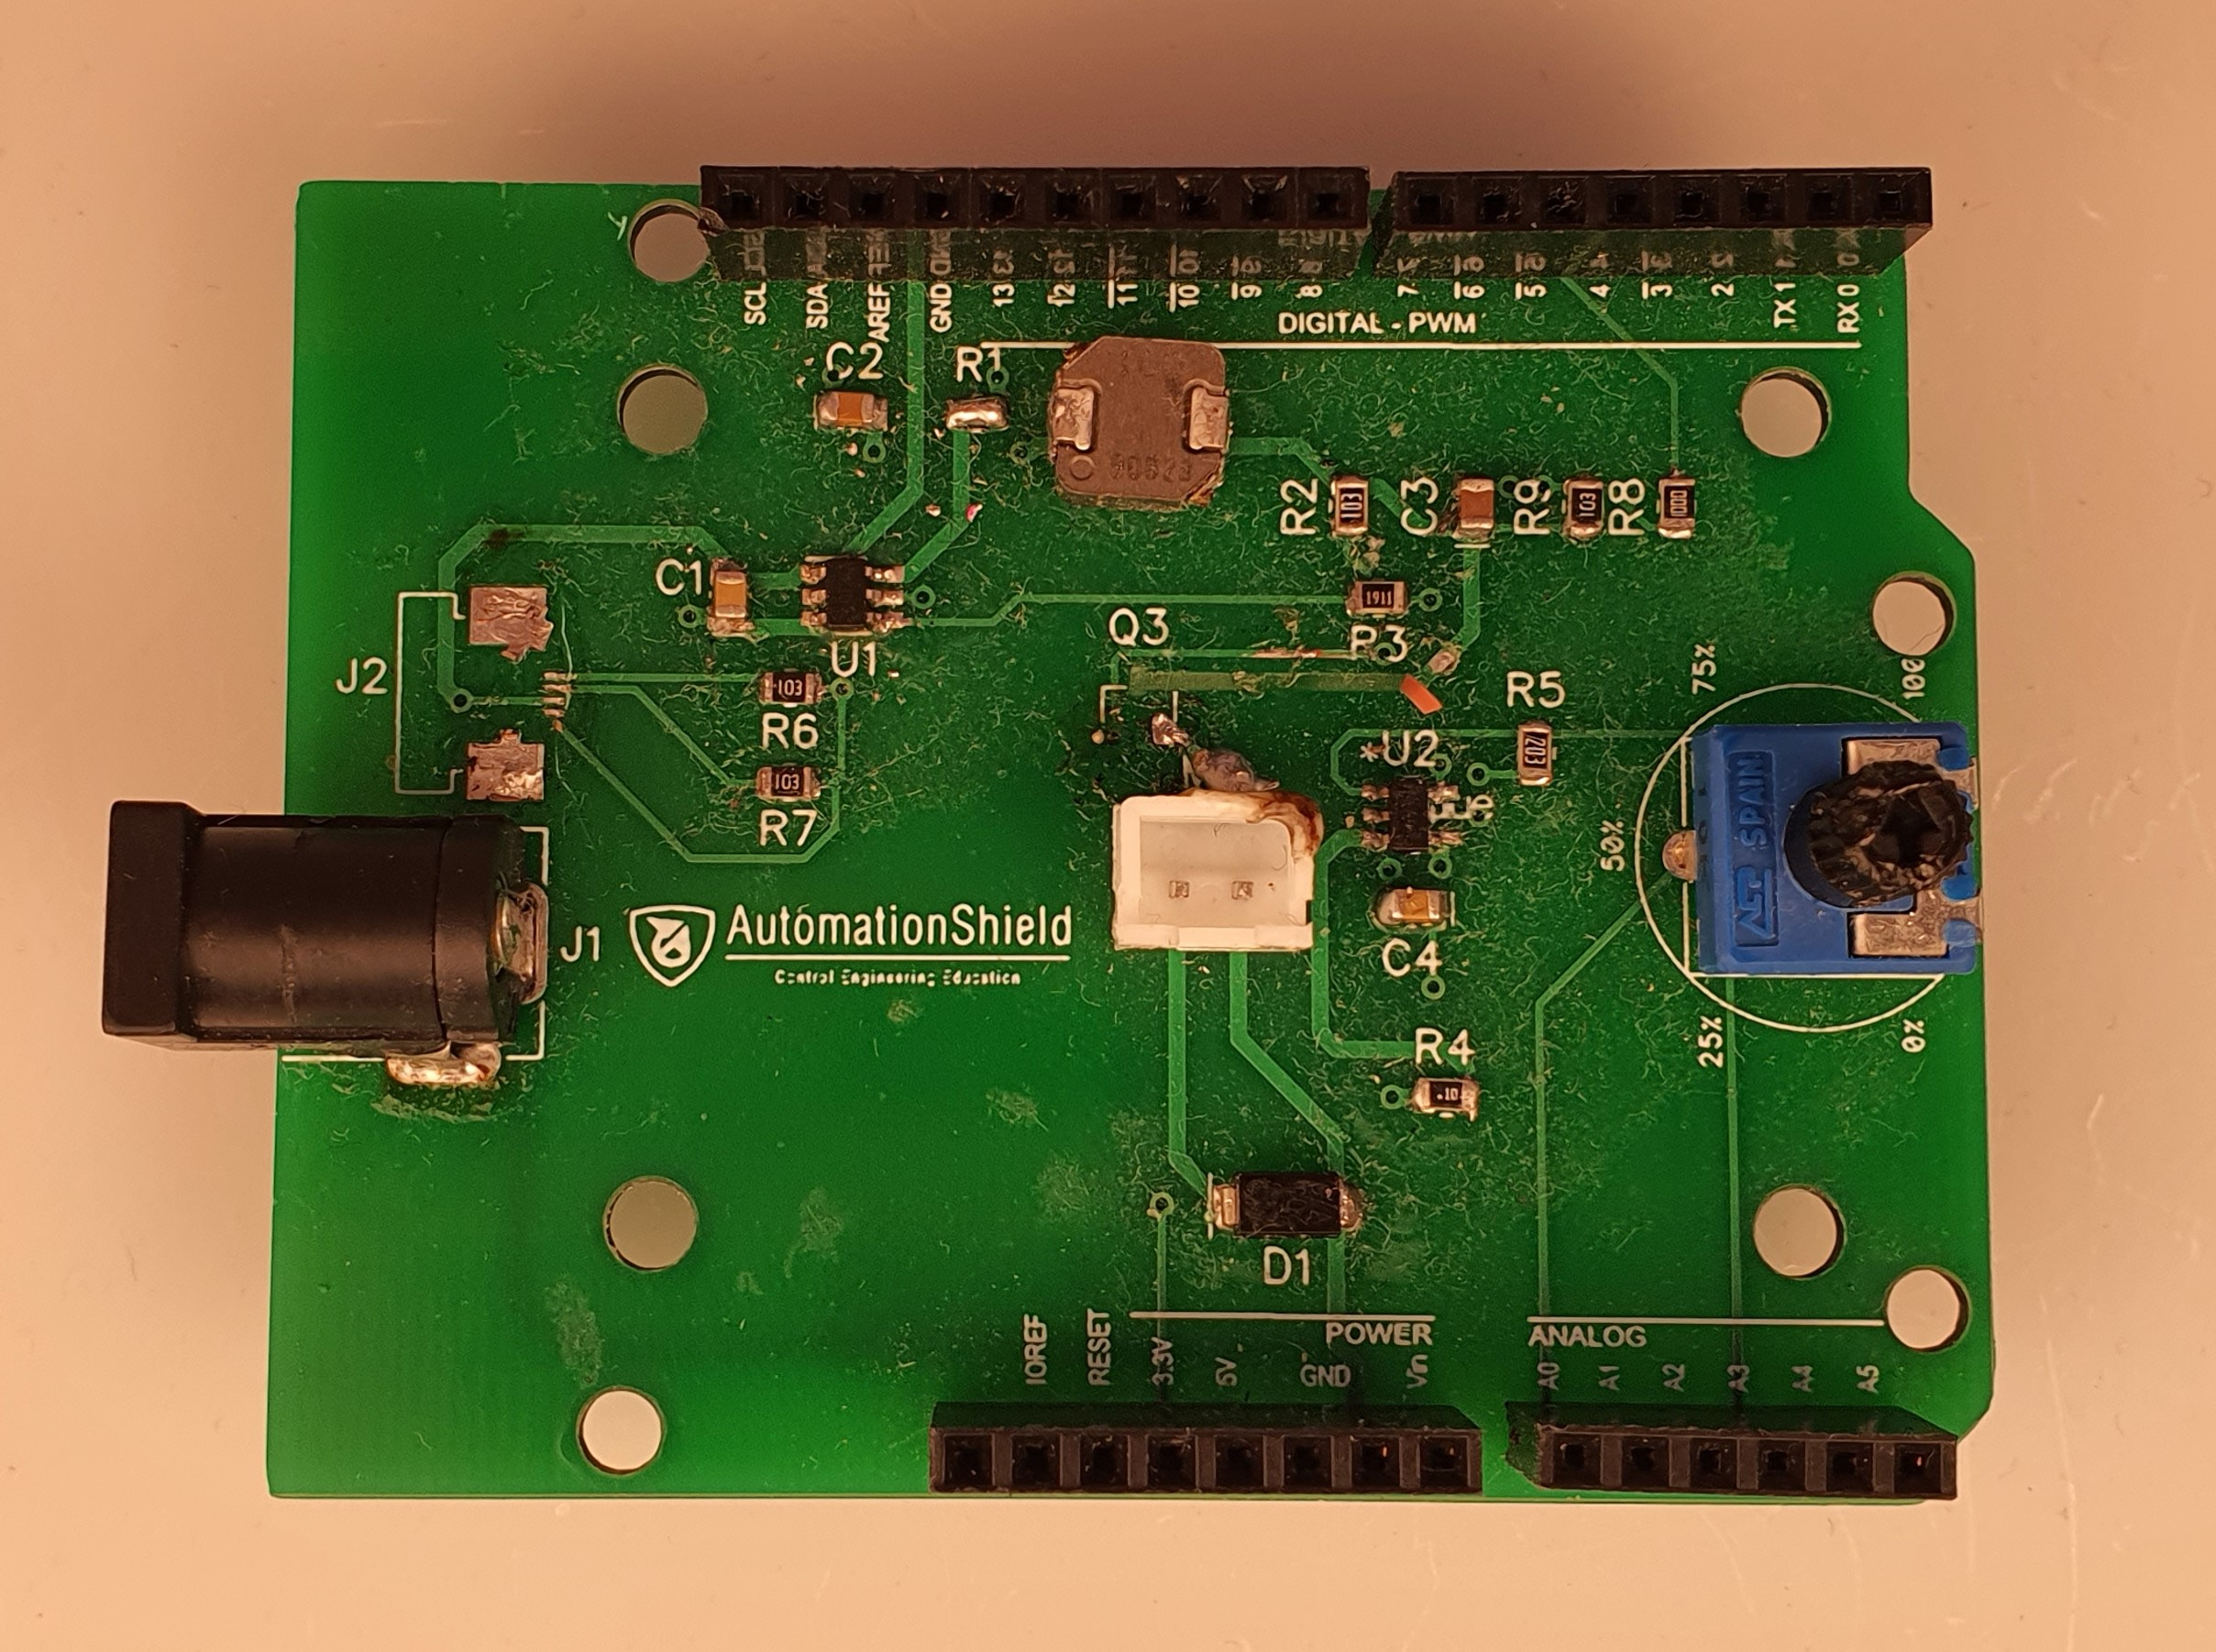
\includegraphics[width=80mm]{obr/oldshield.jpg}

(a)
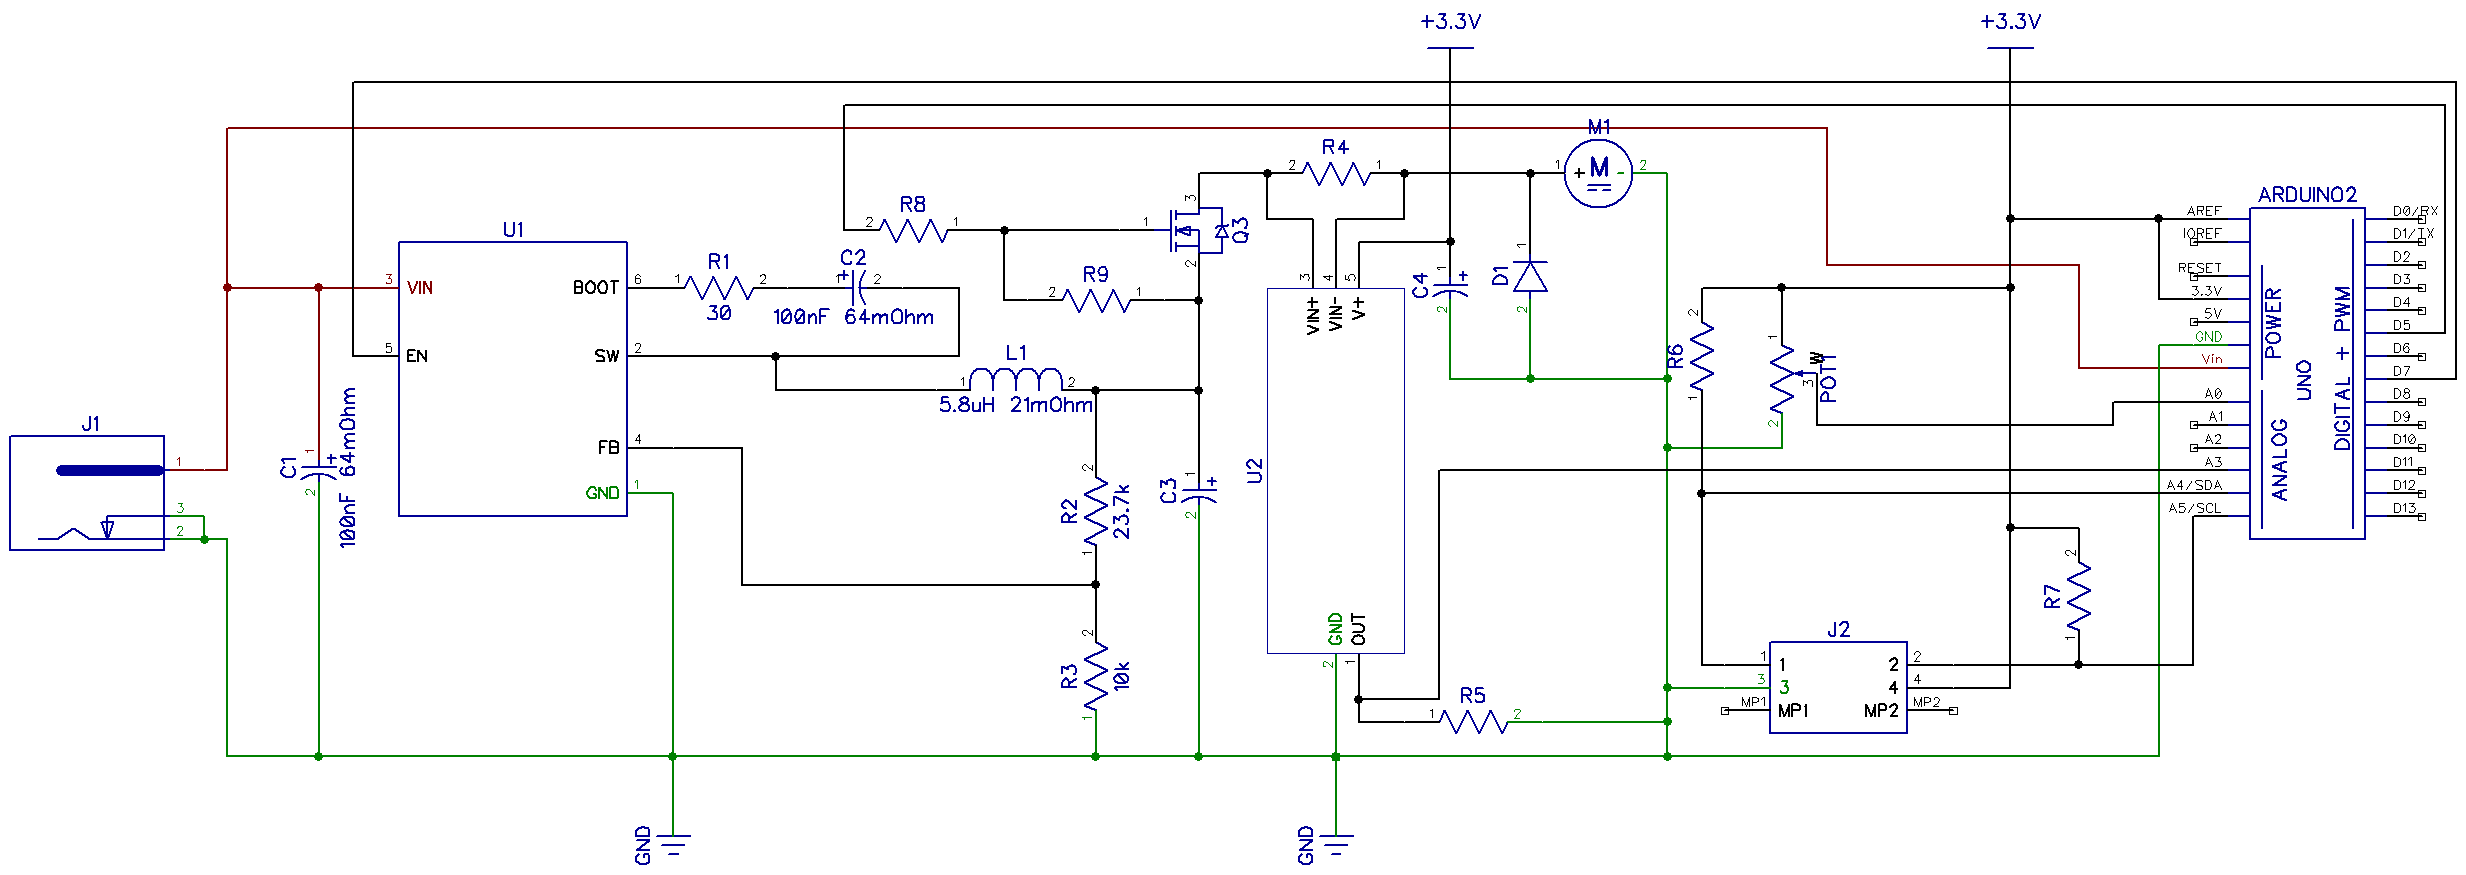
\includegraphics[width=\linewidth]{obr/oldshieldscheme.png}
(b)
\caption{(a) Prvá verzia AeroShieldu. (b) Schéma zapojenia prvej verzie AeroShieldu.}
\label{OBRAZOK 2.1.1}
\end{figure}

\vspace{3cm}

Prvá verzia dosky mala niekoľko nedostatkov, vďaka ktorým bola prakticky nepoužiteľná. Hlavnými nedostatkami boli:

\begin{itemize}
\item neprepojenie pinov komunikácie I2C tj. piny SDA a SCL senzoru hall efektu, ktorý slúži na meranie uhlu natočenia kyvadla,
\item nesprávne zapojenie mosfetu PMW45EN, ktorý ovláda PWM signál idúci do akčného člena,
\item nesprávne umiestnená ochranná dióda na konektoroch akčného člena,
\item nesprávne zapojený obvod s čipom INA169, ktorý slúži na meranie prúdu,
\item neprepojenie nulového konektora shieldu s nulovým konektorom arduina.
\end{itemize}

Základom tejto bakalárskej práce teda bolo najskôr pochopiť jednotlivé časti zapojenia, analizovať chyby a ich následná oprava. V rámci školského projektu bola vytvorená hlavná doska na ktorej sa nachádza väčšina elektroniky, avšak bola vytvorená aj verzia menšej dosky ktorá slúži na fungovanie senzoru hall efektu. Táto doska fungovala bezproblémovo a teda netrebalo nijakým spôsobom meniť jej schému zapojenia viditelnú na obr.\ref{OBRAZOK 2.1.2}.a. Tejto menšej doske sa budeme bližšie venovať v časti\ref{}, no jej podoba je viditelná na obr.\ref{OBRAZOK 2.1.2}.b.


\begin{figure}[!tbh]
\hfill
\subfigure[Schéma zapojenia externej dosky.]{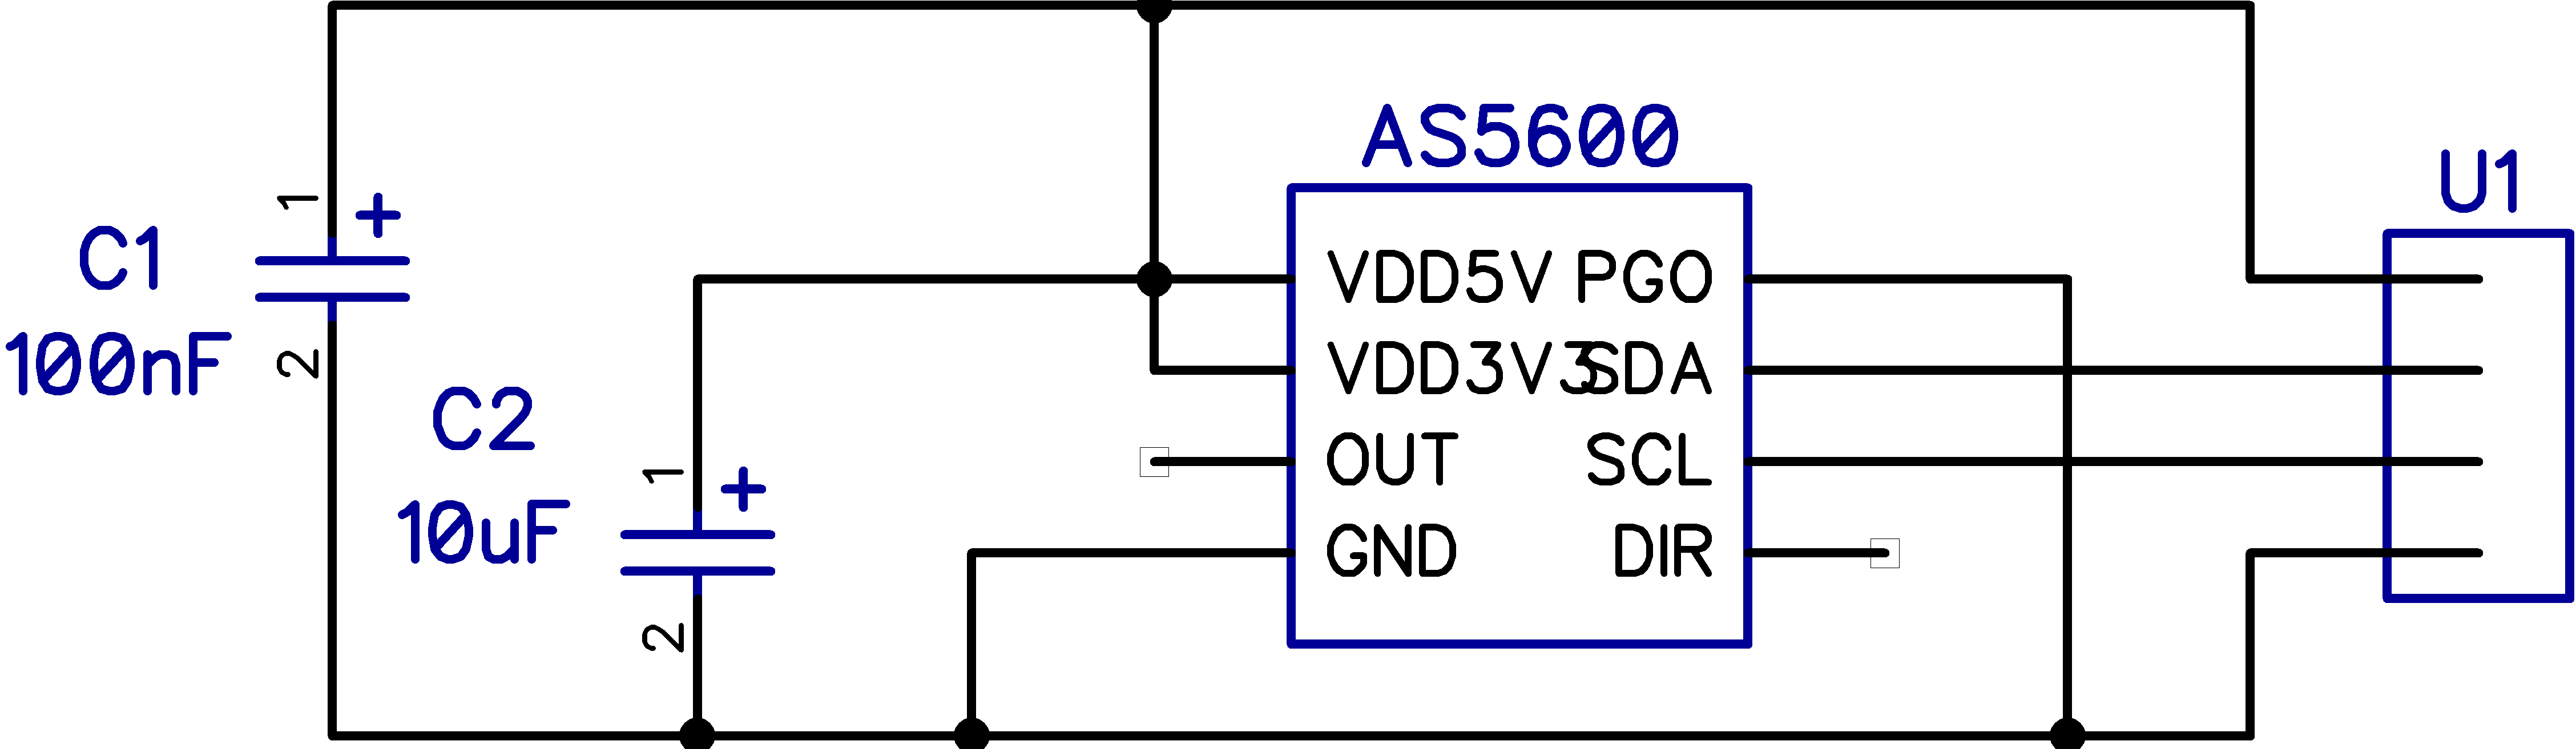
\includegraphics[width=9cm]{obr/as5600.png}}
\hfill
\subfigure[Doska slúžiaca na fungovanie senzoru hall efektu]{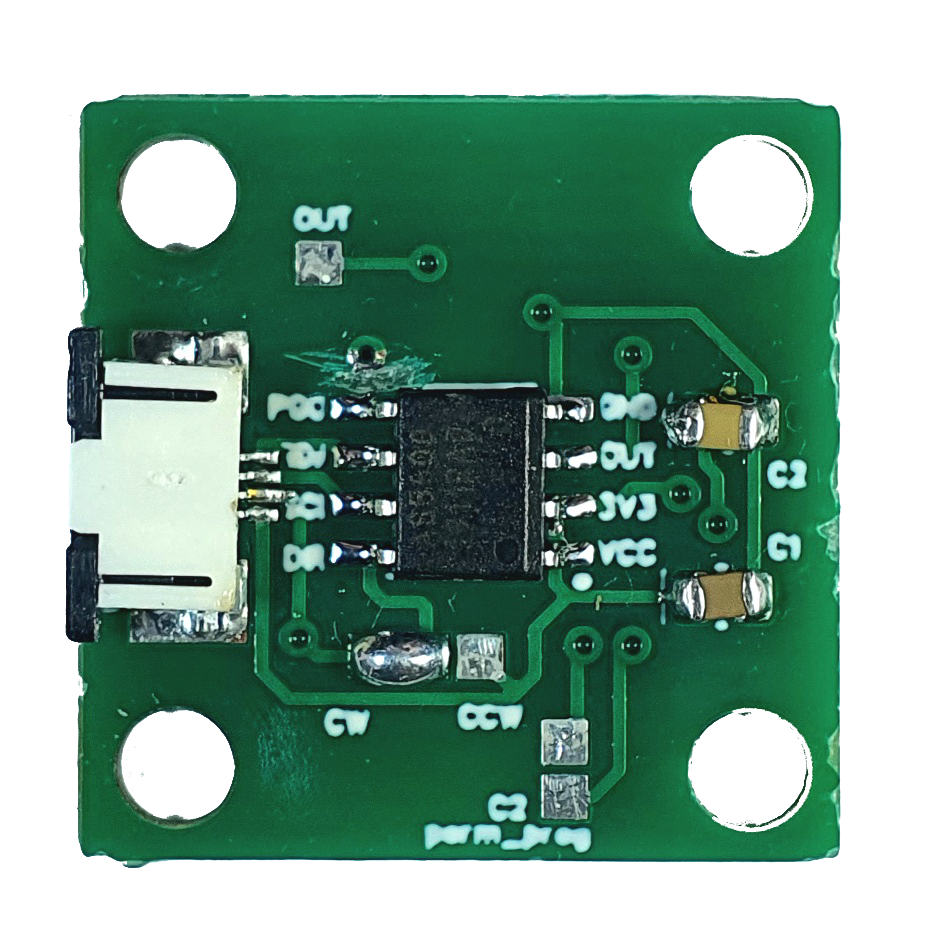
\includegraphics[width=5cm]{obr/fotoBreak.png}}
\hfill
\caption{meranie uhla kyvadla}\label{OBRAZOK 2.1.2}
\end{figure}

\vspace{3cm}


\section{Hardware}
\subsection{Popis súčiastok}

V tejto časti sa bližsie pozrieme na jednotlivé nevyhnutné súčasti zapojenia AeroShieldu. Konkrétne sa jedná o tieto prvky:
\begin{multicols}{2}
\begin{itemize}
\item napájanie
\item ovládanie akčného člena
\item meranie uhla natočenia kyvadla
\item meranie prúdu
    \end{itemize}
    \end{multicols}


\subsubsection{Znižovanie napätia}
\label{nap}

Na správne napájanie akčného člena, motorčeka, potrebujeme napätie v rozmedzí 0-3,7V. Na shield je však privázdané, pomocou koaxiálneho napájacieho konektora, napätie 12V ktoré by motor v priebehu chvíle zničilo. Potrebujeme preto spôsob ako znížiť privádzané napätie, no súčastne neznížiť privádzaný prúd potrebný na pohon motorčeka. Na tieto účely slúži takzvaný buck converter alebo konvertor na zníženie napätia. Hlavnou Časťou konvertora je čip TPS56339 od výrobcu Texas Instruments obr.\ref{OBRAZOK 2.1}.b. Znižovanie napätia funguje za pomoci dvoch integrovaných N-kanálových 70-m$\Omega$ a 35-m$\Omega$ high-side mosfetov\footnote[4]{N-kanálový mosfet je typ mosfetu, v ktorom tok prúdu nastáva kvôli pohybujucím sa, záporne nabitým elektrónom. "High-side" znamená, že prúd prechádza z napájania, cez mosfet do záťaže a potom do zeme} a dalších komponentov. Celkový prevádzkový prúd zariadenia je približne 98$\upmu$A, keď funguje bez spínania a bez záťaže. Keď je zariadenie vypnuté, napájací prúd je približne 3$\upmu$A a zariadenie umožňuje nepretržitý výstupný prúd do 3 A\cite{buckobr}.

\begin{figure}[!tbh]
\hfill
\subfigure[Schéma zapojenia konvertora napätia.]{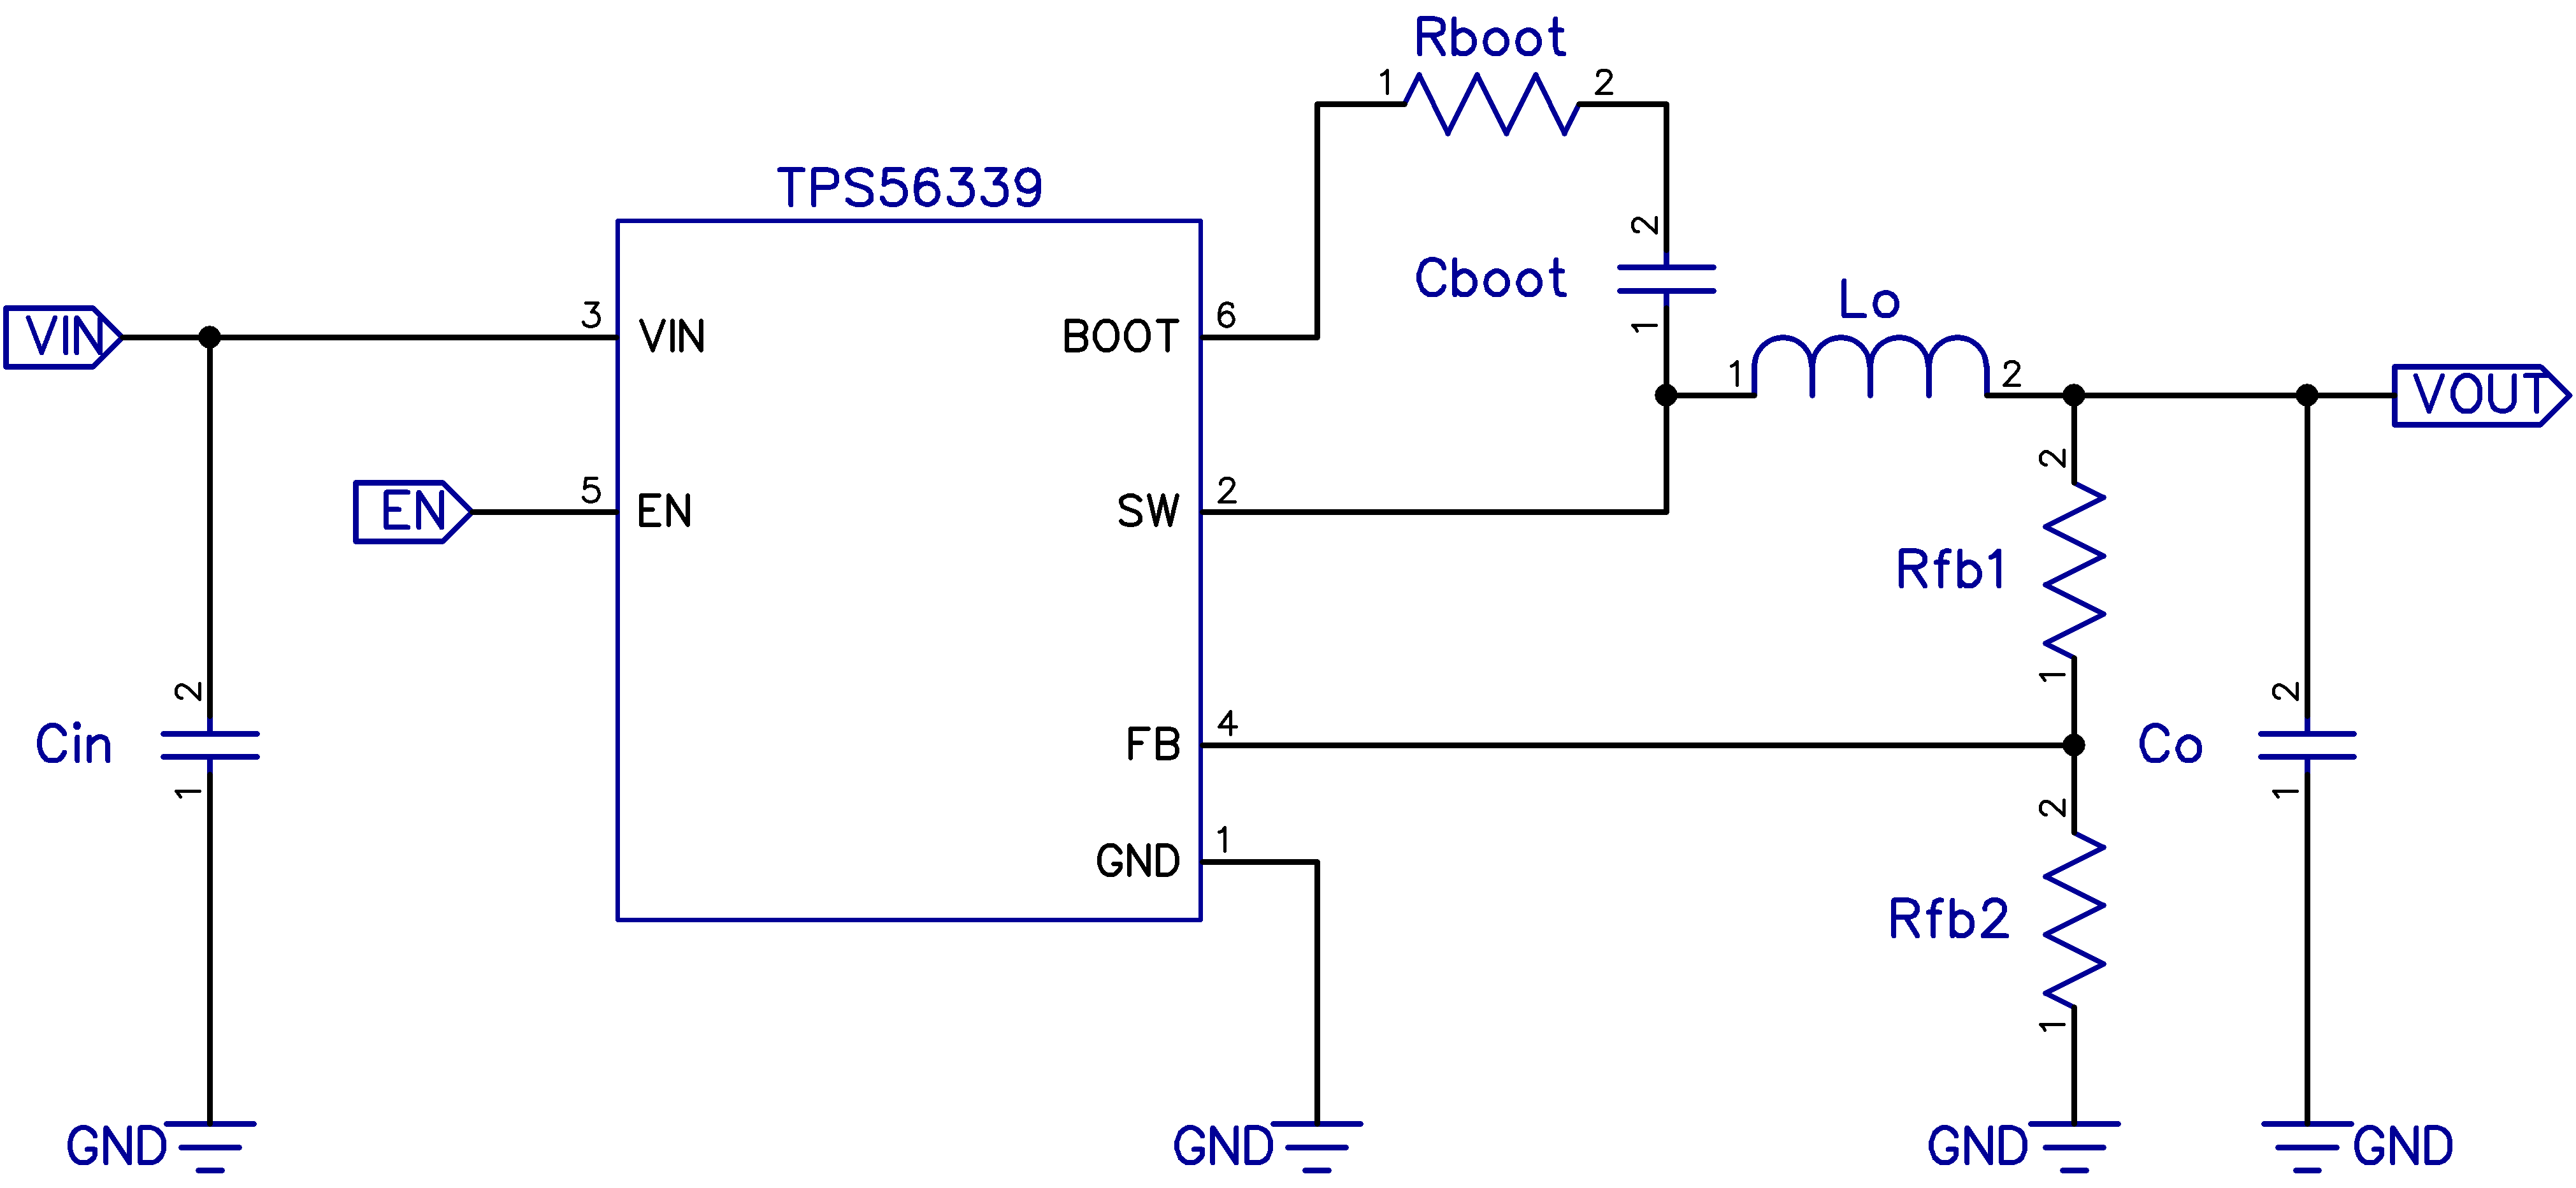
\includegraphics[width=9cm]{obr/schemaBuck.png}}
\hfill
\subfigure[{čip TPS56339\cite{buckobr}}]{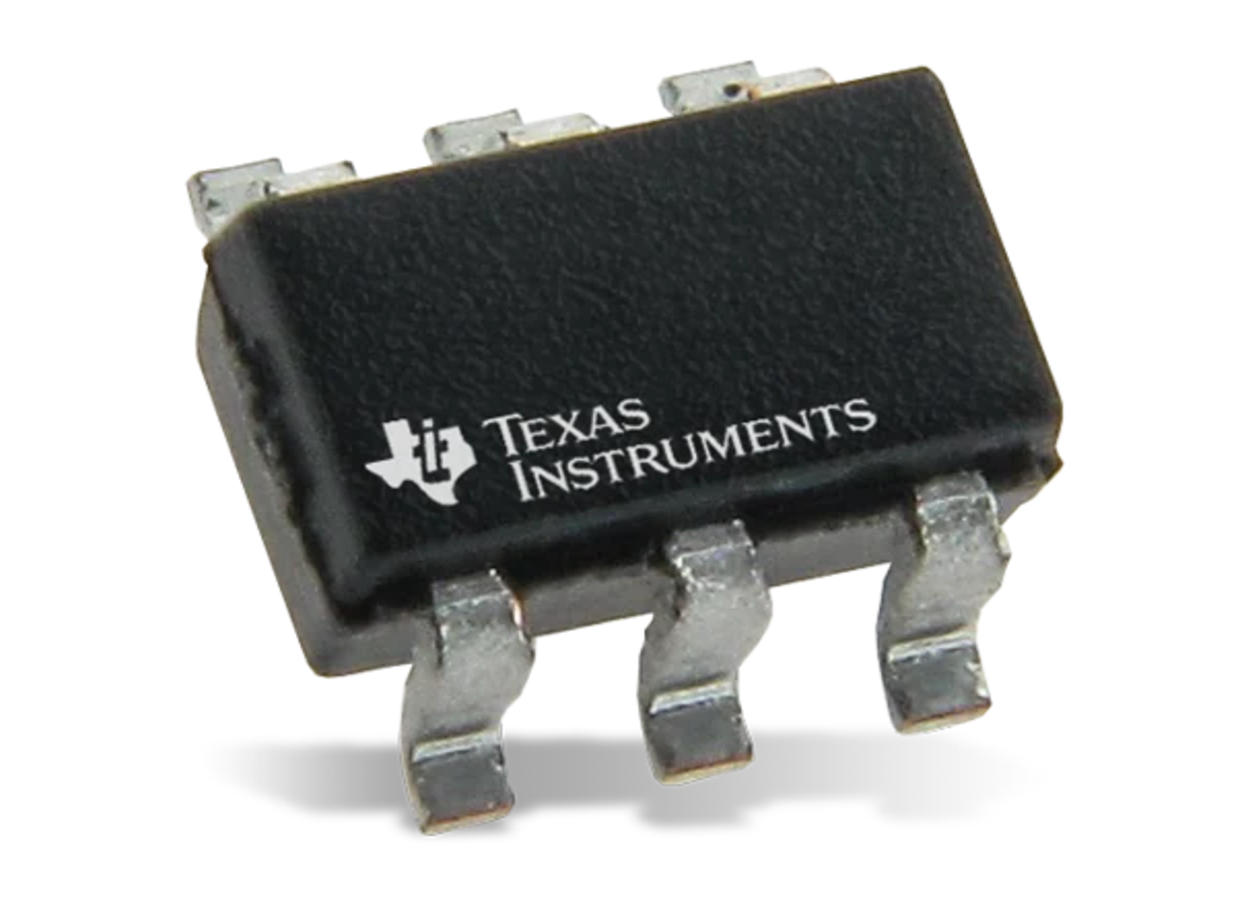
\includegraphics[width=5cm]{obr/cip.eps}}
\hfill
\caption{buck converter}\label{OBRAZOK 2.1}
\end{figure}

 Na čip je privádzané napätie 12V ktoré sa pomocou zapojenia, vididelného na schéme obr.\ref{OBRAZOK 2.1}.a, znižuje na napätie 3,7V. Napájanie motora musí byť realizované externe pomocou koaxiálneho napájacieho konektora, z dôvodu vysokého prúdu odoberaného motorom počas vysokého zaťaženia. Rovnaký konektor sa síce nachádza aj na doske Arduino UNO a pomocou VIN pinu sa dajú napájať napätím 0-12V aj iné zariadenia, avšak tento pin je napojený na diódu obmedzujúcu prúd na 1A\cite{ampere}\cite{ampere2}.



\subsubsection{akčný člen}
\label{akcclen}

Ako akčný člen AeroShieldu je použitý 7mm, 3,7V motorček na jednosmerný prúd, bez jadra. “coreless motor“ alebo motor bez jadra je motor s cievkou navinutou samou na sebe a nie na železe\cite{coreless}. Takéto jadro ale samé o sebe nie je veľmi pevné a nedrží dobre tvar, preto sa častokrát zalieva epoxidom. Stator je vyrobený z magnetov na báze vzácnych zemín, ako je neodým alebo SmCo(samárium-kobalt), ktoré sa nachádzajú vo vnútri bezjadrového rotora.

Takýto motor ponúka mnoho výhod oproti motoru so železným jadrom. Tým že jadro v sebe nemá železo, výrazne sa znižuje hmotnosť a tým aj zotrvačnosť rotora, čo je dôležité pre naše použitie kedy potrebujeme dosahovať vysokú akceleráciu a rýchle spomalenie rotora. Ďalšou výhodou je fakt že nedochádza k stratám na železe a tým pádom sa účinnosť takýchto motorov blíži až ku 90\%-\cite{5545147}. Motor resp. otáčky motora sú riadené pomocou impulzovej šírkovej modulácie(PWM) a tieto impulzy do motoru prechádzajú cez N-kanálový mosfet PMV45EN2 od výrobcu Nexperia\cite{pmv}.



\begin{figure}[!tbh]
\hfill
\subfigure[Schéma zapojenia motorčeka.]{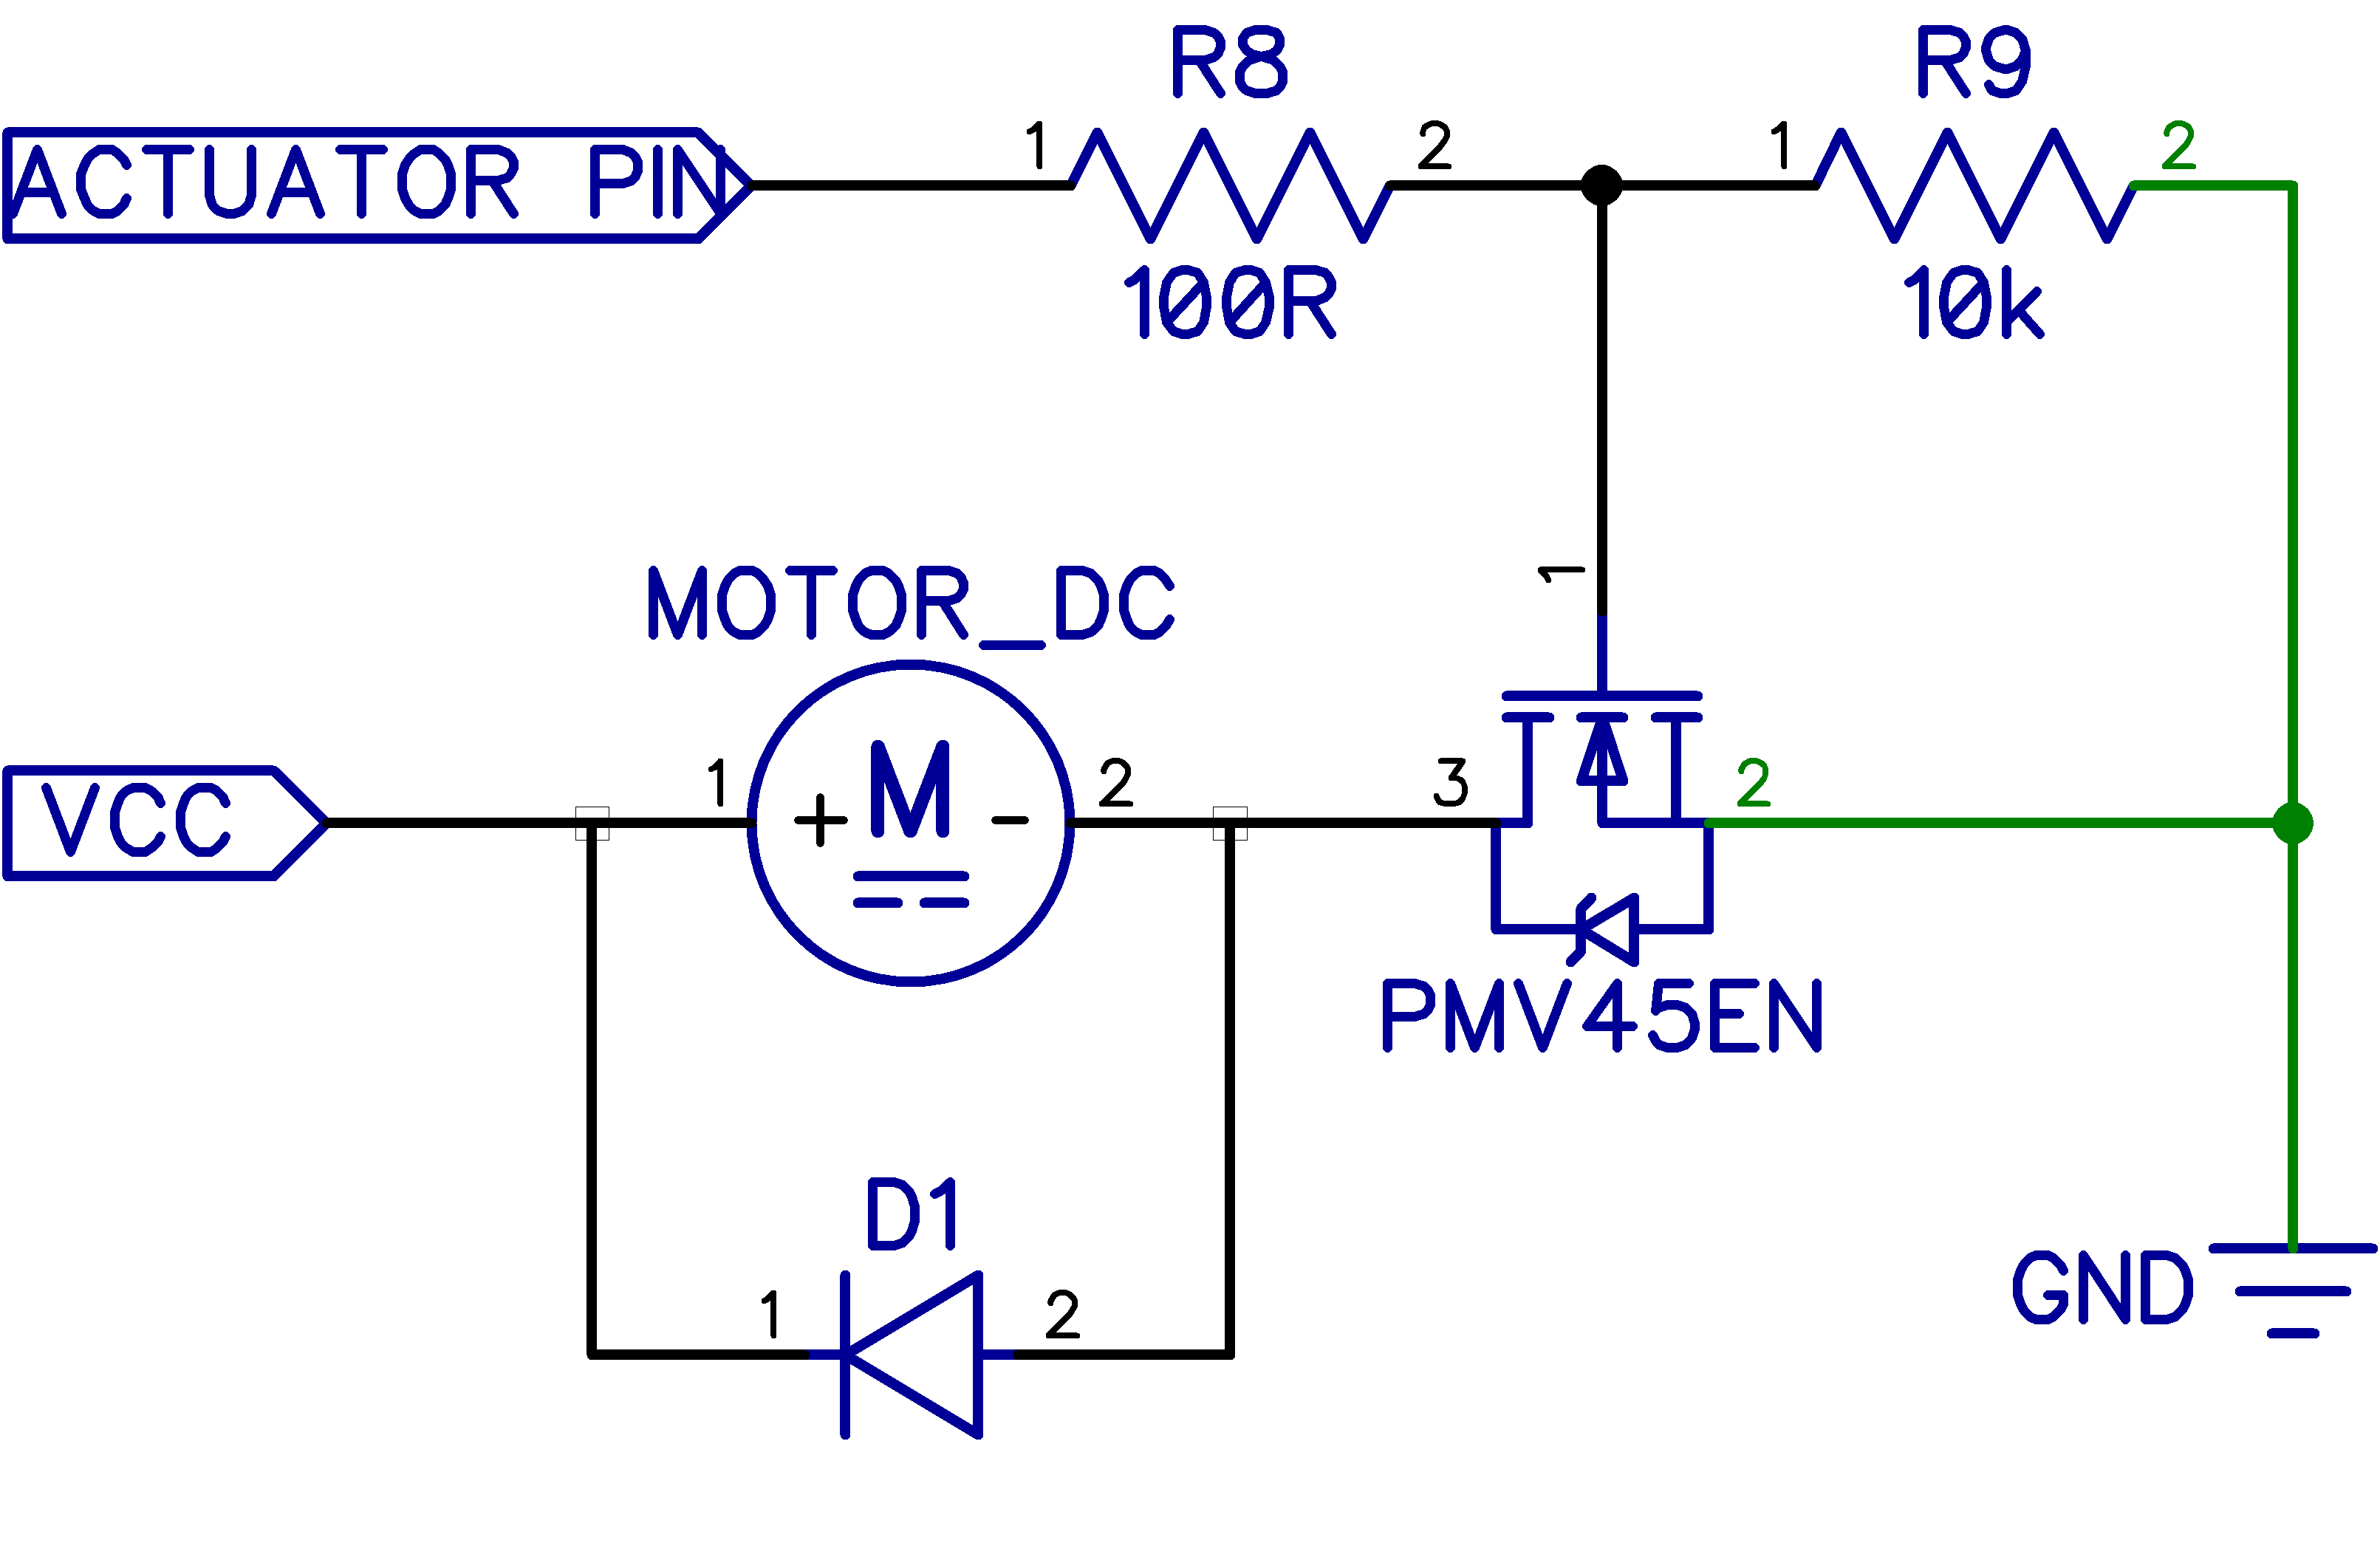
\includegraphics[width=7cm]{obr/MotorScheme.png}}
\hfill
\subfigure[{Motorček\cite{corelessMotor}}]{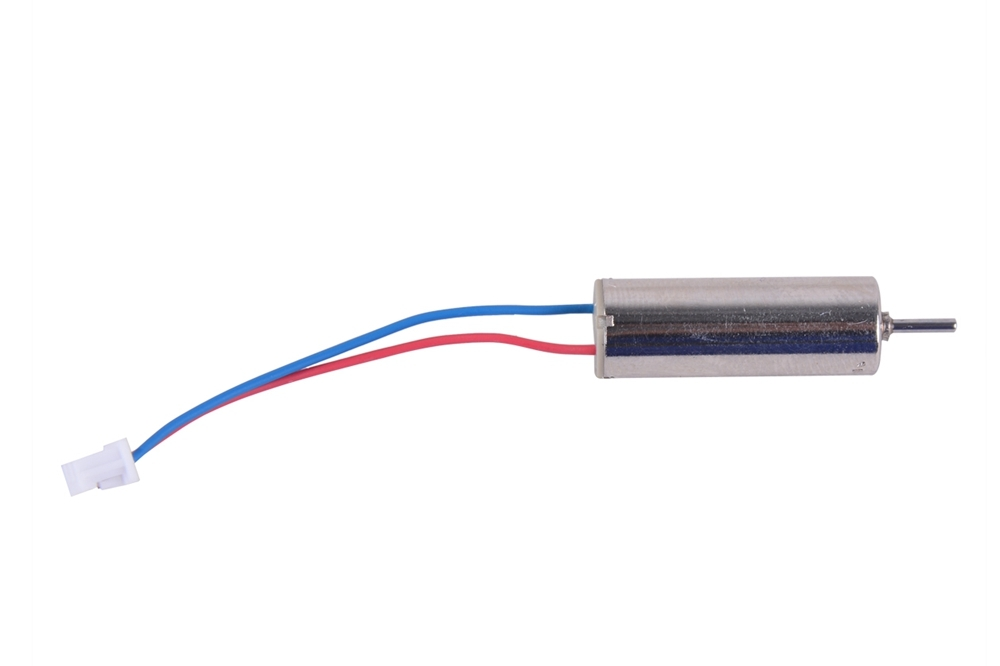
\includegraphics[width=7cm]{obr/coreless.jpg}}
\hfill
\caption{akčný člen}\label{OBRAZOK 2.3}
\end{figure}


\subsubsection{meranie prúdu}
\label{merprud}

Pre čo najpresnejšie ovládanie akčného člena sústavy, motora, je dobré vedieť nie len napätie, ktorým je motor ovládaný, ale aj prúd, ktorý motor odoberá. Na tieto účely sa používajú monitory prúdu, takzvané "current shunt monitors". V AeroShielde je použitý snímač INA169NA/250 od výrobcu Texas Instruments obr.\ref{OBRAZOK 2.3}.b.

INA169 funguje na základe zaznamenávania zmien napätia na stranách shunt rezistora obr.\ref{OBRAZOK 2.3}.a. Na základe nameraného úbytku napätia, vysiela senzor poďla nami zvoleného stupňa zosilnenia, prúd, ktorý je ďalej pomocou rezistoru $R_{l}$ premenený na napätie s maximálnou hodnotou $V_{OUTMAX} = V_{IN-} - 0.5V $.

 Prúd $I_{s}$ odoberaný motorom, vypočítame pomocou vzorca $I_{s} = \dfrac{V_{OUT}\: x \: 1k\Omega}{R_{s} \: x \: R_{l}} $ kde $V_{OUT}$ je napätie namerané na výstupe, 1k$\Omega$ je konštanta vnútorných odporov senzoru, $R_{s}$ je hodnota shunt rezistora v $\Omega$ a $R_{l}$ je hodnota rezistora na výstupe, taktiež v $\Omega$\cite{INA}.

\begin{figure}[!tbh]
\hfill
\subfigure[Schéma zapojenia snímača prúdu.]{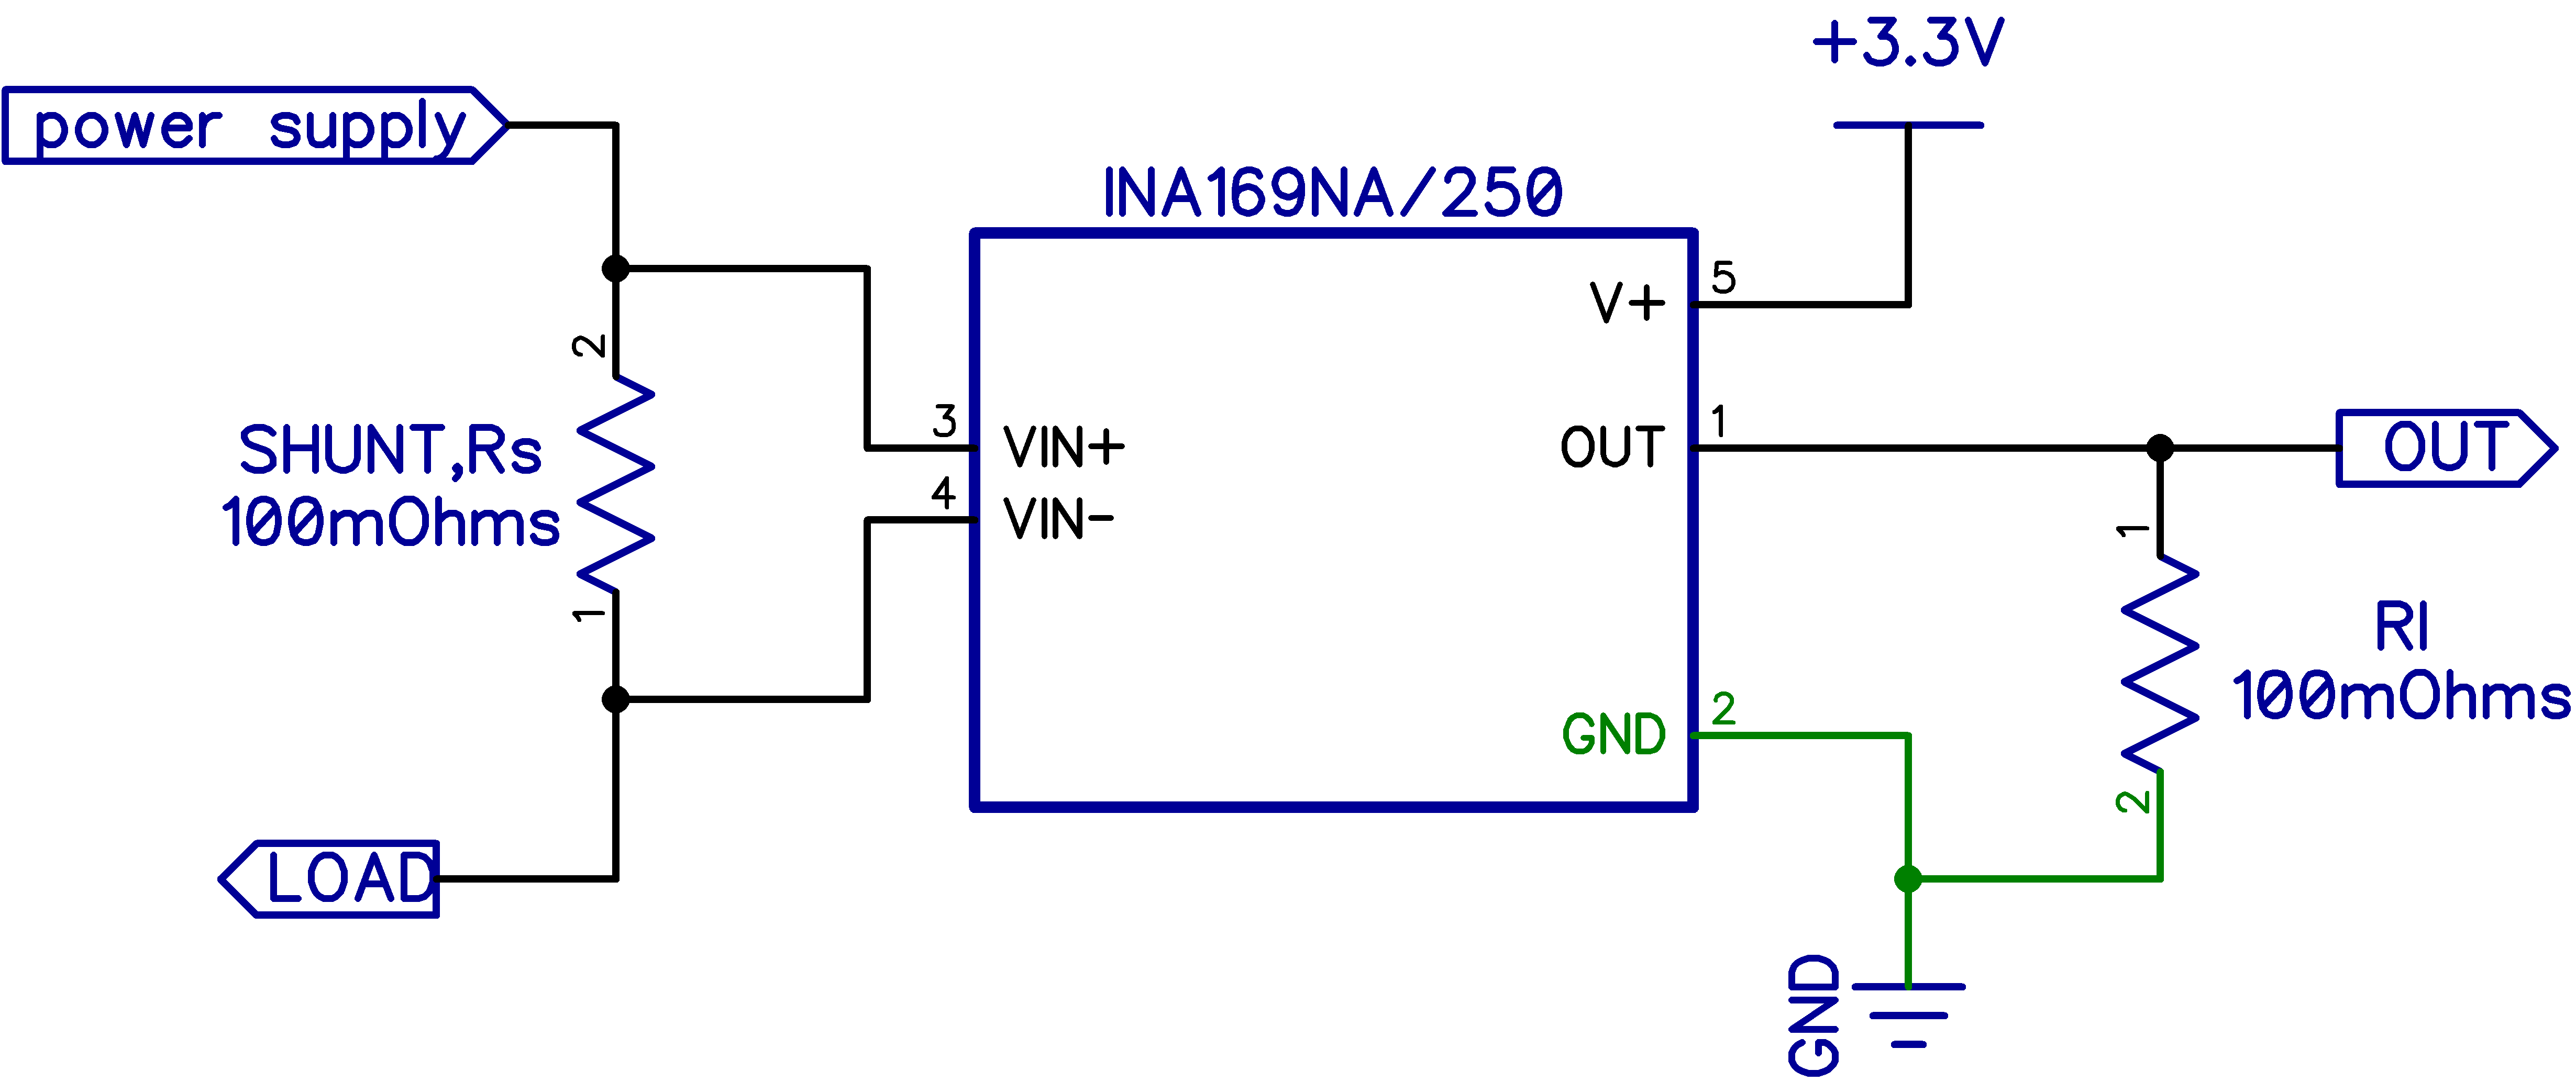
\includegraphics[width=9cm]{obr/INAschema.png}}
\hfill
\subfigure[{Senzor INA169NA/250\cite{INAobr}}]{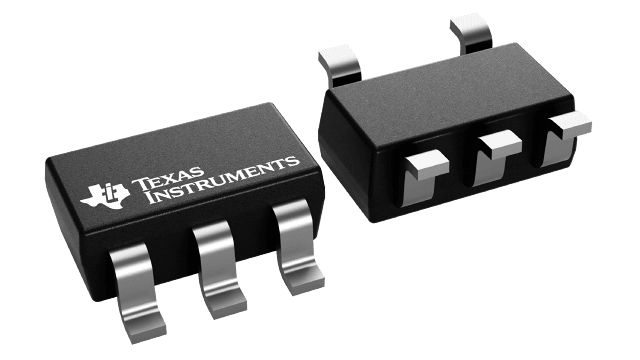
\includegraphics[width=6cm]{obr/ina.png}}
\hfill
\caption{meranie prúdu}\label{OBRAZOK 2.3}
\end{figure}


\label{Hall}
\pagebreak

\subsubsection{meranie uhla kyvadla}
\label{meruhl}

Na správne fungovanie AeroShieldu je dôležité vedieť s vysokou presnosťou merať uhol naklonenia kyvadla. Na tento účel sme si zvolili meranie uhlu bezkontaktnou formou, pomocou snímača na princípe hallovho javu. Hallov jav vieme opísať ako vznik priečneho elektrického poľa v pevnom materiáli, keď ním preteká elektrický prúd a tento materiál je umiestnený v magnetickom poli, ktoré je kolmé na prúd\cite{Hall}. Toto elektrické pole resp. vznik elektrického potenciálu vieme detegovať a na základe jeho zmeny vieme určit rotáciu kyvadla. V kyvadle je na konci horizontálneho ramena umiestnený špeciálny magnet kruhového tvaru ktorý je polarizovaný naprieč prierezom magnetu.

Ako senzor na meranie hallovho efektu je použitý AS5600 od výrobcu OSRAM obr.\ref{OBRAZOK 2.2}.b. Signály prichádzajúce zo snímača sa najprv zosilnia, následne sú filtrované a prechádzajú konverziou pomocou analógovo-digitálneho prevodníkom (ADC). Snímaná je aj intenzita magnetického poľa, ktorá sa ďalej používa na
automatické riadenie zosilnenia(AGC), ktoré slúži na kompenzáciu teploty a veľkosti magnetického poľa.

Na výber sú dva typy výstupu a to analógový výstup alebo digitálny výstup s kódovaním PWM. Senzor má taktiež aj možnosti interného programovania pomocou rozhrania I2C.
V našom prípade používame 12-bitový analógový výstup s rozlíšením 0°5'16". Toto rozlíšenie nám umožnuje s vysokou presnosťou kontrolovať naklonenie kyvadla a na základe získaných informácii ovplyvňovať fungovanie akčného členu sústavy. Schéma zapojenia čipu na meranie uhlu môžeme vidieť na obr.\ref{OBRAZOK 2.2}.a.



\begin{figure}[!tbh]
\hfill
\subfigure[Schéma zapojenia čipu na meranie uhlu.]{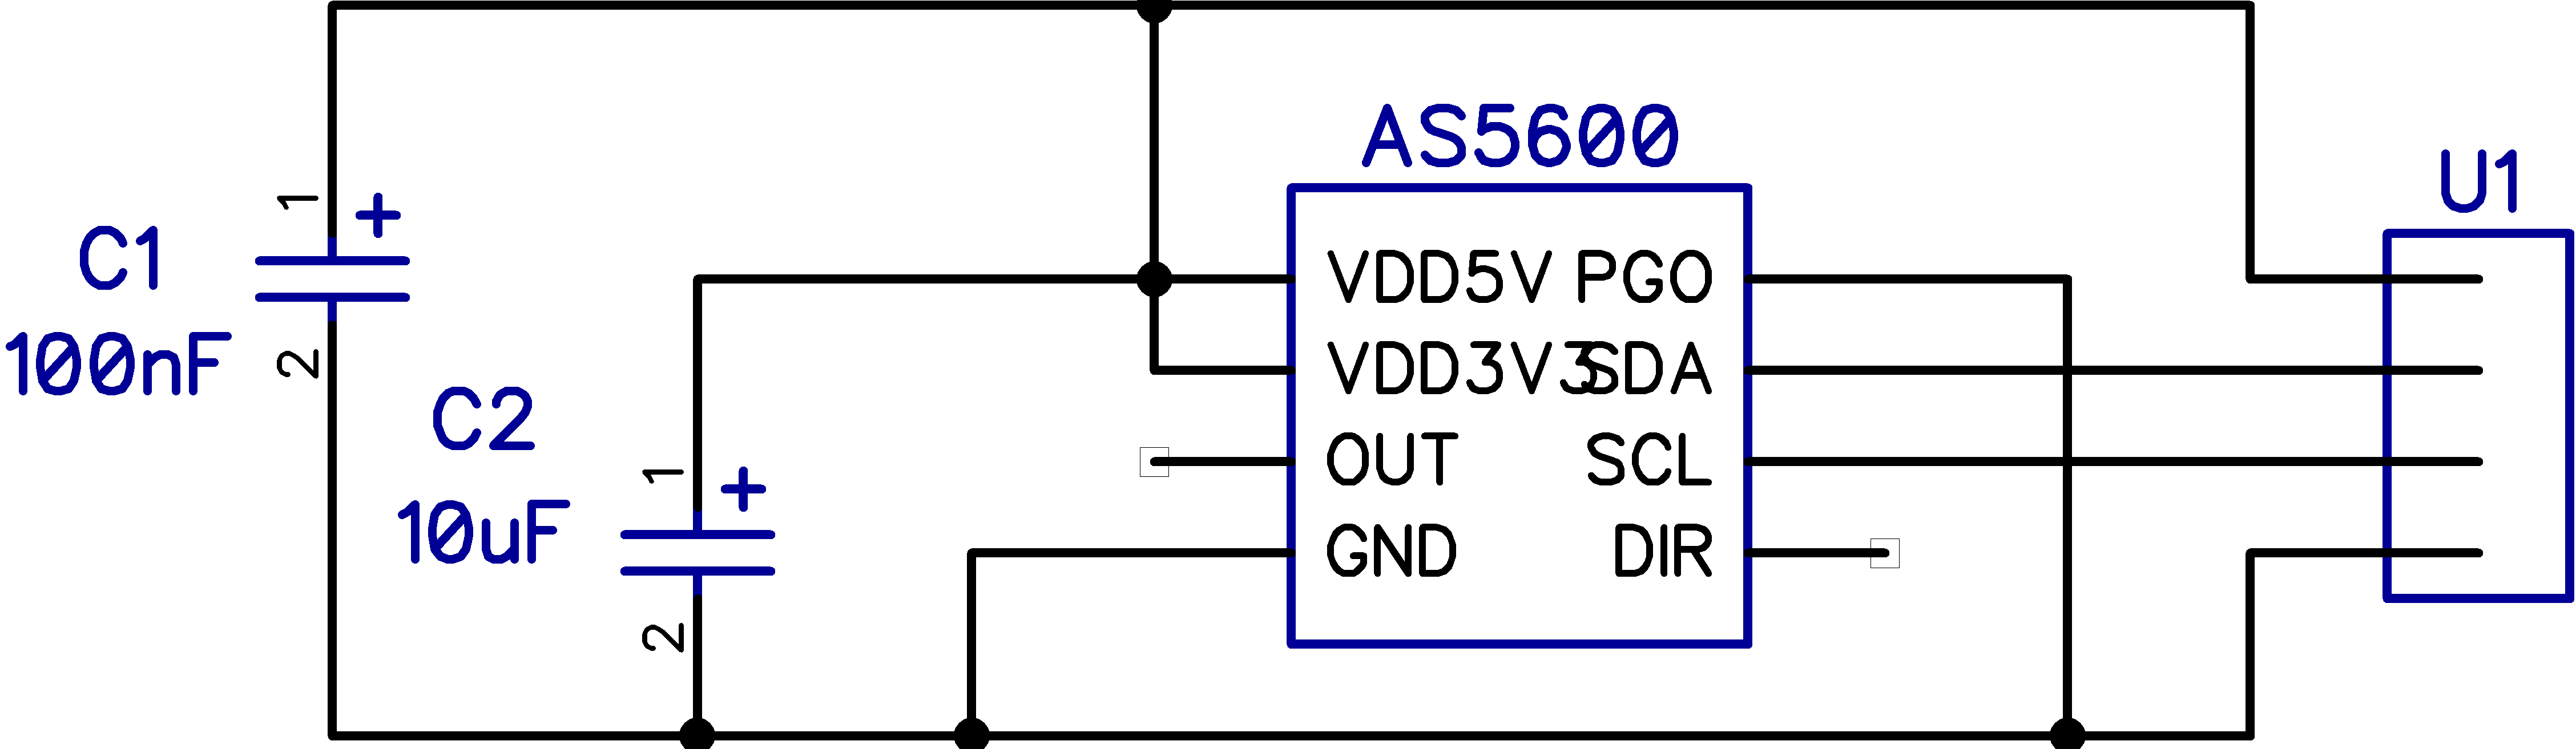
\includegraphics[width=10cm]{obr/as5600.png}}
\hfill
\subfigure[{čip AS5600\cite{As5600obr}}]{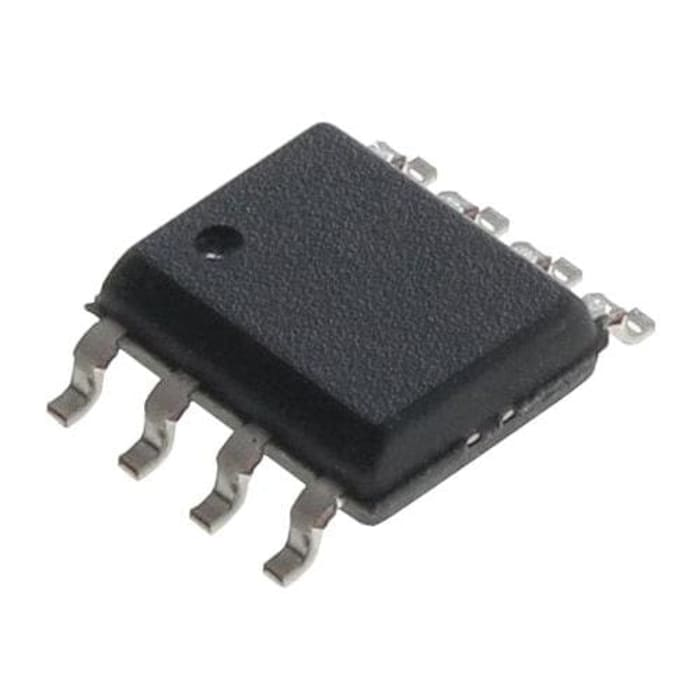
\includegraphics[width=4cm]{obr/hall.jpg}}
\hfill
\caption{meranie uhla kyvadla}\label{OBRAZOK 2.2}
\end{figure}

\newpage


\subsection{Schéma zapojenia}

Všetky schémy zapojenia boli tvorené v bezplatnej verzii programu DipTrace. DipTrace slúži ako prostredie na tvorbu elektrotechnických schém, potrebných pre výrobu dosiek plošných spojov, ako aj pre účely prehľadnosti zapojenia komponentov na týchto doskách. Program v sebe zahŕňa časť pre tvorbu samotných komponentov, pokial sa tieto už nenachádzajú v niektorej z knižníc programu, časť kde sa tvoria schémy zapojenia a časť na tvorbu dosiek plošných spojov.

Nie všetky komponenty potrebné na tvorbu AeroShieldu boli zahrnuté v knižniciach DipTracu, avšak tieto komponenty sa nachádzali na stiahnutie na stránkach výrobcov odkiaľ boli importované do novej knižnice, slúžiacej na účely tvorby schémy AeroShieldu. Do programu bola taktiež vložená knižnica AutomationShieldu ktorá má v sebe najčastejšie používané komponenty. Pri tvorbe schémy zapojenia sa najskôr všetky potrebné komponenty umiestnia na štvorčekovú plochu a približne sa určí ích poloha. Jednotlivé komponenty majú podobu elektrotechnických značiek a každý komponent má ku sebe priradené reálne vlastnosti daného dielu(veľkosť, zapojenie, dĺžka pinov a iné).

Polohu volíme takú, aby schéma bola čo najprehladnejšia a komponenty ktoré sú medzi sebou prepojené, boli čo najbližšie pri sebe. Akonáhle máme všetky komponenty uložené začneme s ich postupným prepájaním. Pri zapájaní jednotlivých komponentov sa riadime katalógovými listami jednotlivých komponentov, v ktorých býva zväčša aj návrh ich zapojenia.

Veľmi dobrou vlastnosťou pogramu DipTrace je možnosť zafarbovania jednotlivých elektrických spojení, rozličnými farbami a názvami. Tento fakt nám veľmi uľahčuje na prvý pohľad rozoznať napríklad elektrické spojenia zeme- 0V zelená, fázové spojenia- 3,3V červená obr.\ref{OBRAZOK 2.3}. Na schéme zapojenia môžeme vidieť všetky komponenty, potrebné na správne fungovanie AeroShieldu. Názvy komponentov sú uvádzané základnými značkami
\begin{multicols}{3}
    \begin{itemize}
\item R- Rezistor
\item C- Kapacitor
\item J- Konektor
\item U- Mikročip
\item L- Cievka
\item D- Dióda
\item M- Motor
    \end{itemize}
    \end{multicols}


\begin{figure}[!tbh]
\includegraphics[width=\textwidth]{obr/aeroSchema.png}
\caption{Schéma zapojenia AeroShieldu}\label{OBRAZOK 2.3}
\end{figure}

\subsection{Doska plošných spojov}

Po návrhu a kontrole schém zapojenia sa schémy dalej spracovávajú do podoby dosky plošných spojov. Schémy exportujeme do programu DipTrace PCB v ktorom máme následne niekoľko možností postupu. Jednotlivé komponenty sa nám už zobrazujú v reálnej podobe, takže vidíme ich veľkosť a rozmiestnenie pinov na pájkovanie.

Po prenesení schém do DipTrace PCB, sú jednotlivé komponenty rozhádzané a nemajú žiadne logické rozloženie. Program ponúka možnosť automatického zoradenia komponentov na vyhradenej ploche, avšak táto funkcia komponenty uložila nie podľa našich potrieb a teda, využili sme možnosť manuálneho umiestnenia jednotlivých komponentov. Pri pohybovaní jednotlivými komponentami môžeme vidieť čiary, ktoré symbolizujú prepojenia s ostatnými komponentami a vďaka tomu vieme komponenty logicky poukladať.

Po zvolení optimálneho rozmiestnenia komponentov treba jednotlivé piny poprepájať cestami, ktoré nám nahrádzajú funkciu káblov. Máme možnosť zvoliť automatické rozmiestnenie ciest alebo ich manuálnu tvorbu. V našom prípade sme zvolili manuálnu tvorbu ciest, pretože ich vieme čo najlepšie optimalizovať.

Tvorba ciest má niekolko pravidiel, avšak najdôležitejšie z nich je že jednotlivé cesty ktoré v schéme zapojenia nie su prepojené, sa nemôžu križovať inak dôjde k ich vzájomnému vyskratovaniu. Z toho dôvodu treba niekedy cestu priviesť na druhú stranu dosky plošných spojov kde v jej pokračovaní neprekáža iná cesta. Na tento účel sa používajú vodivé diery, takzvané via, spájajúce obe strany dosky.

Pri výroby dosky sa taktiež myslelo na montáž držiaku kyvadla, pre ktoré boli vytvorené 4 diery na jeho následné prichytenie pomocou skrutiek. Finálna verzia hlavnej dosky je na obr.\ref{OBRAZOK 2.4}. Zhotovená bola aj menšia doska tzv. breakout board, slúžiaca na meranie uhlu kyvadla, ktorá je na obr.\ref{OBRAZOK 2.6}.

\begin{figure}[!tbh]
\hfill
\subfigure[Vrchná strana breakout boardu]{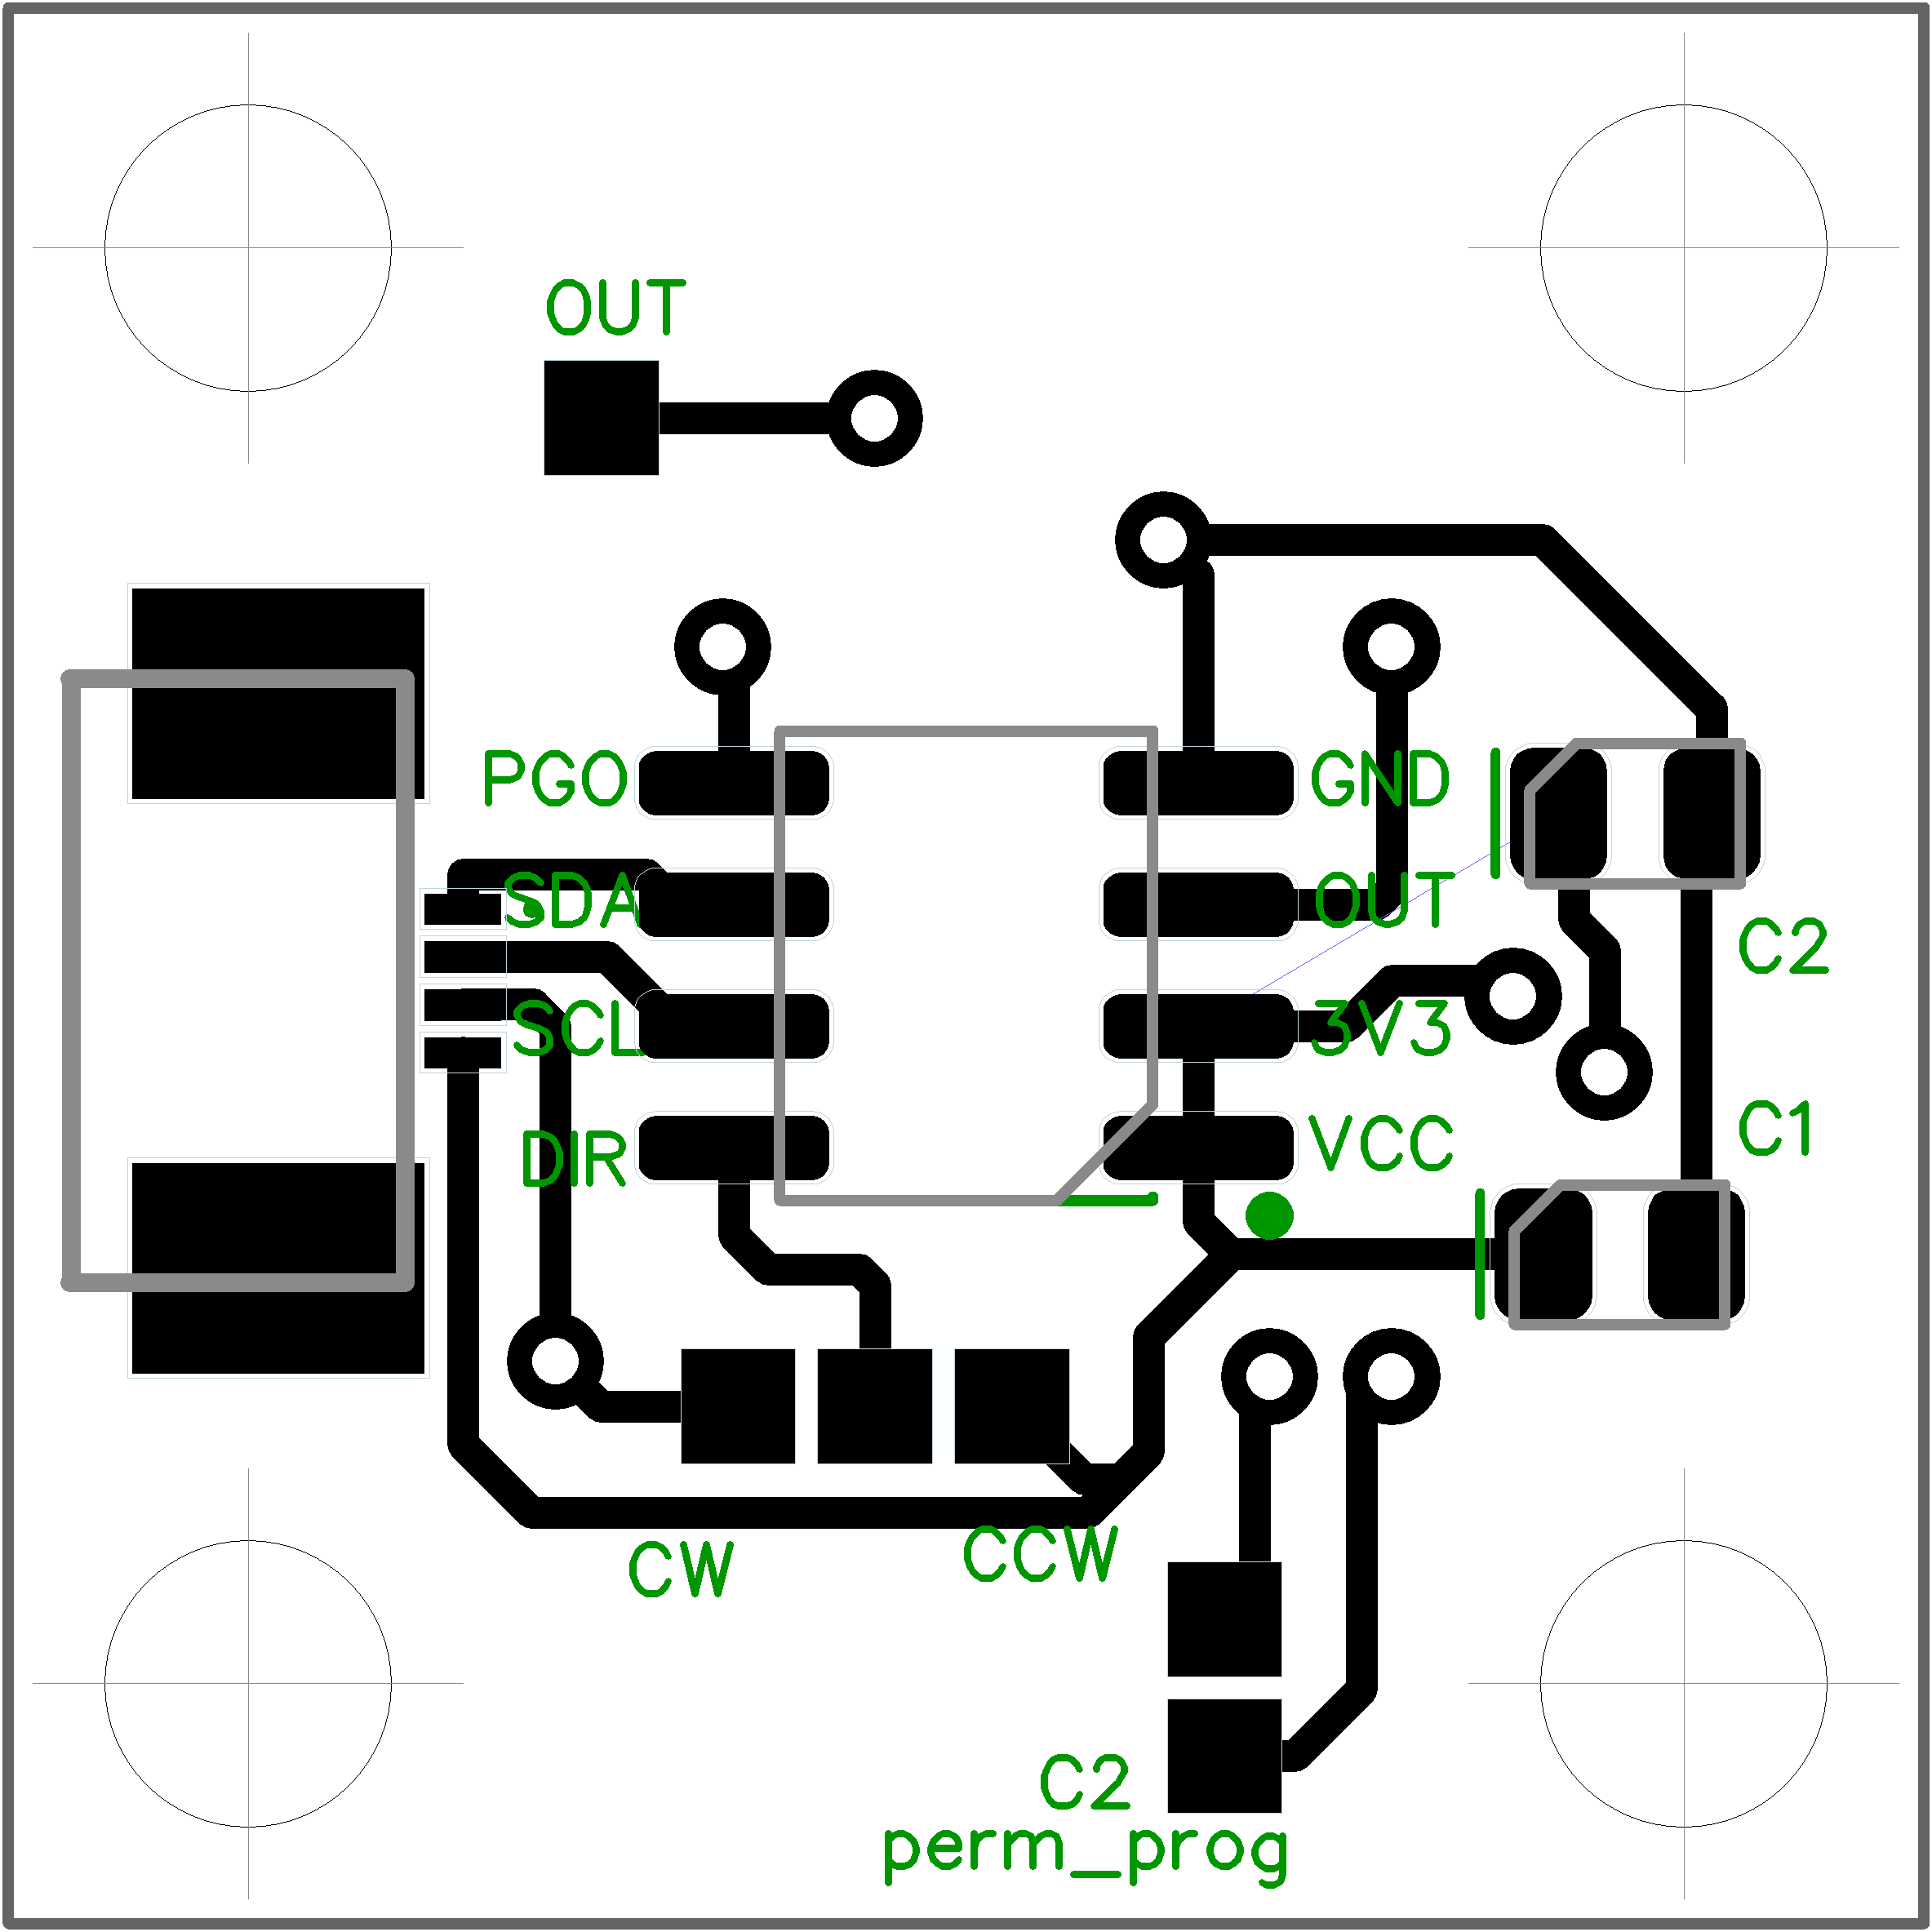
\includegraphics[width=7cm]{obr/breakoutTOP.png}}
\hfill
\subfigure[Spodná strana breakout boardu]{
\includegraphics[width=7cm]{obr/breakoutbottom.png}}
\hfill
\caption{Vedlajšia doska AeroShieldu- breakout board}\label{OBRAZOK 2.6}
\end{figure}

\begin{figure}[!tbh]
\centering
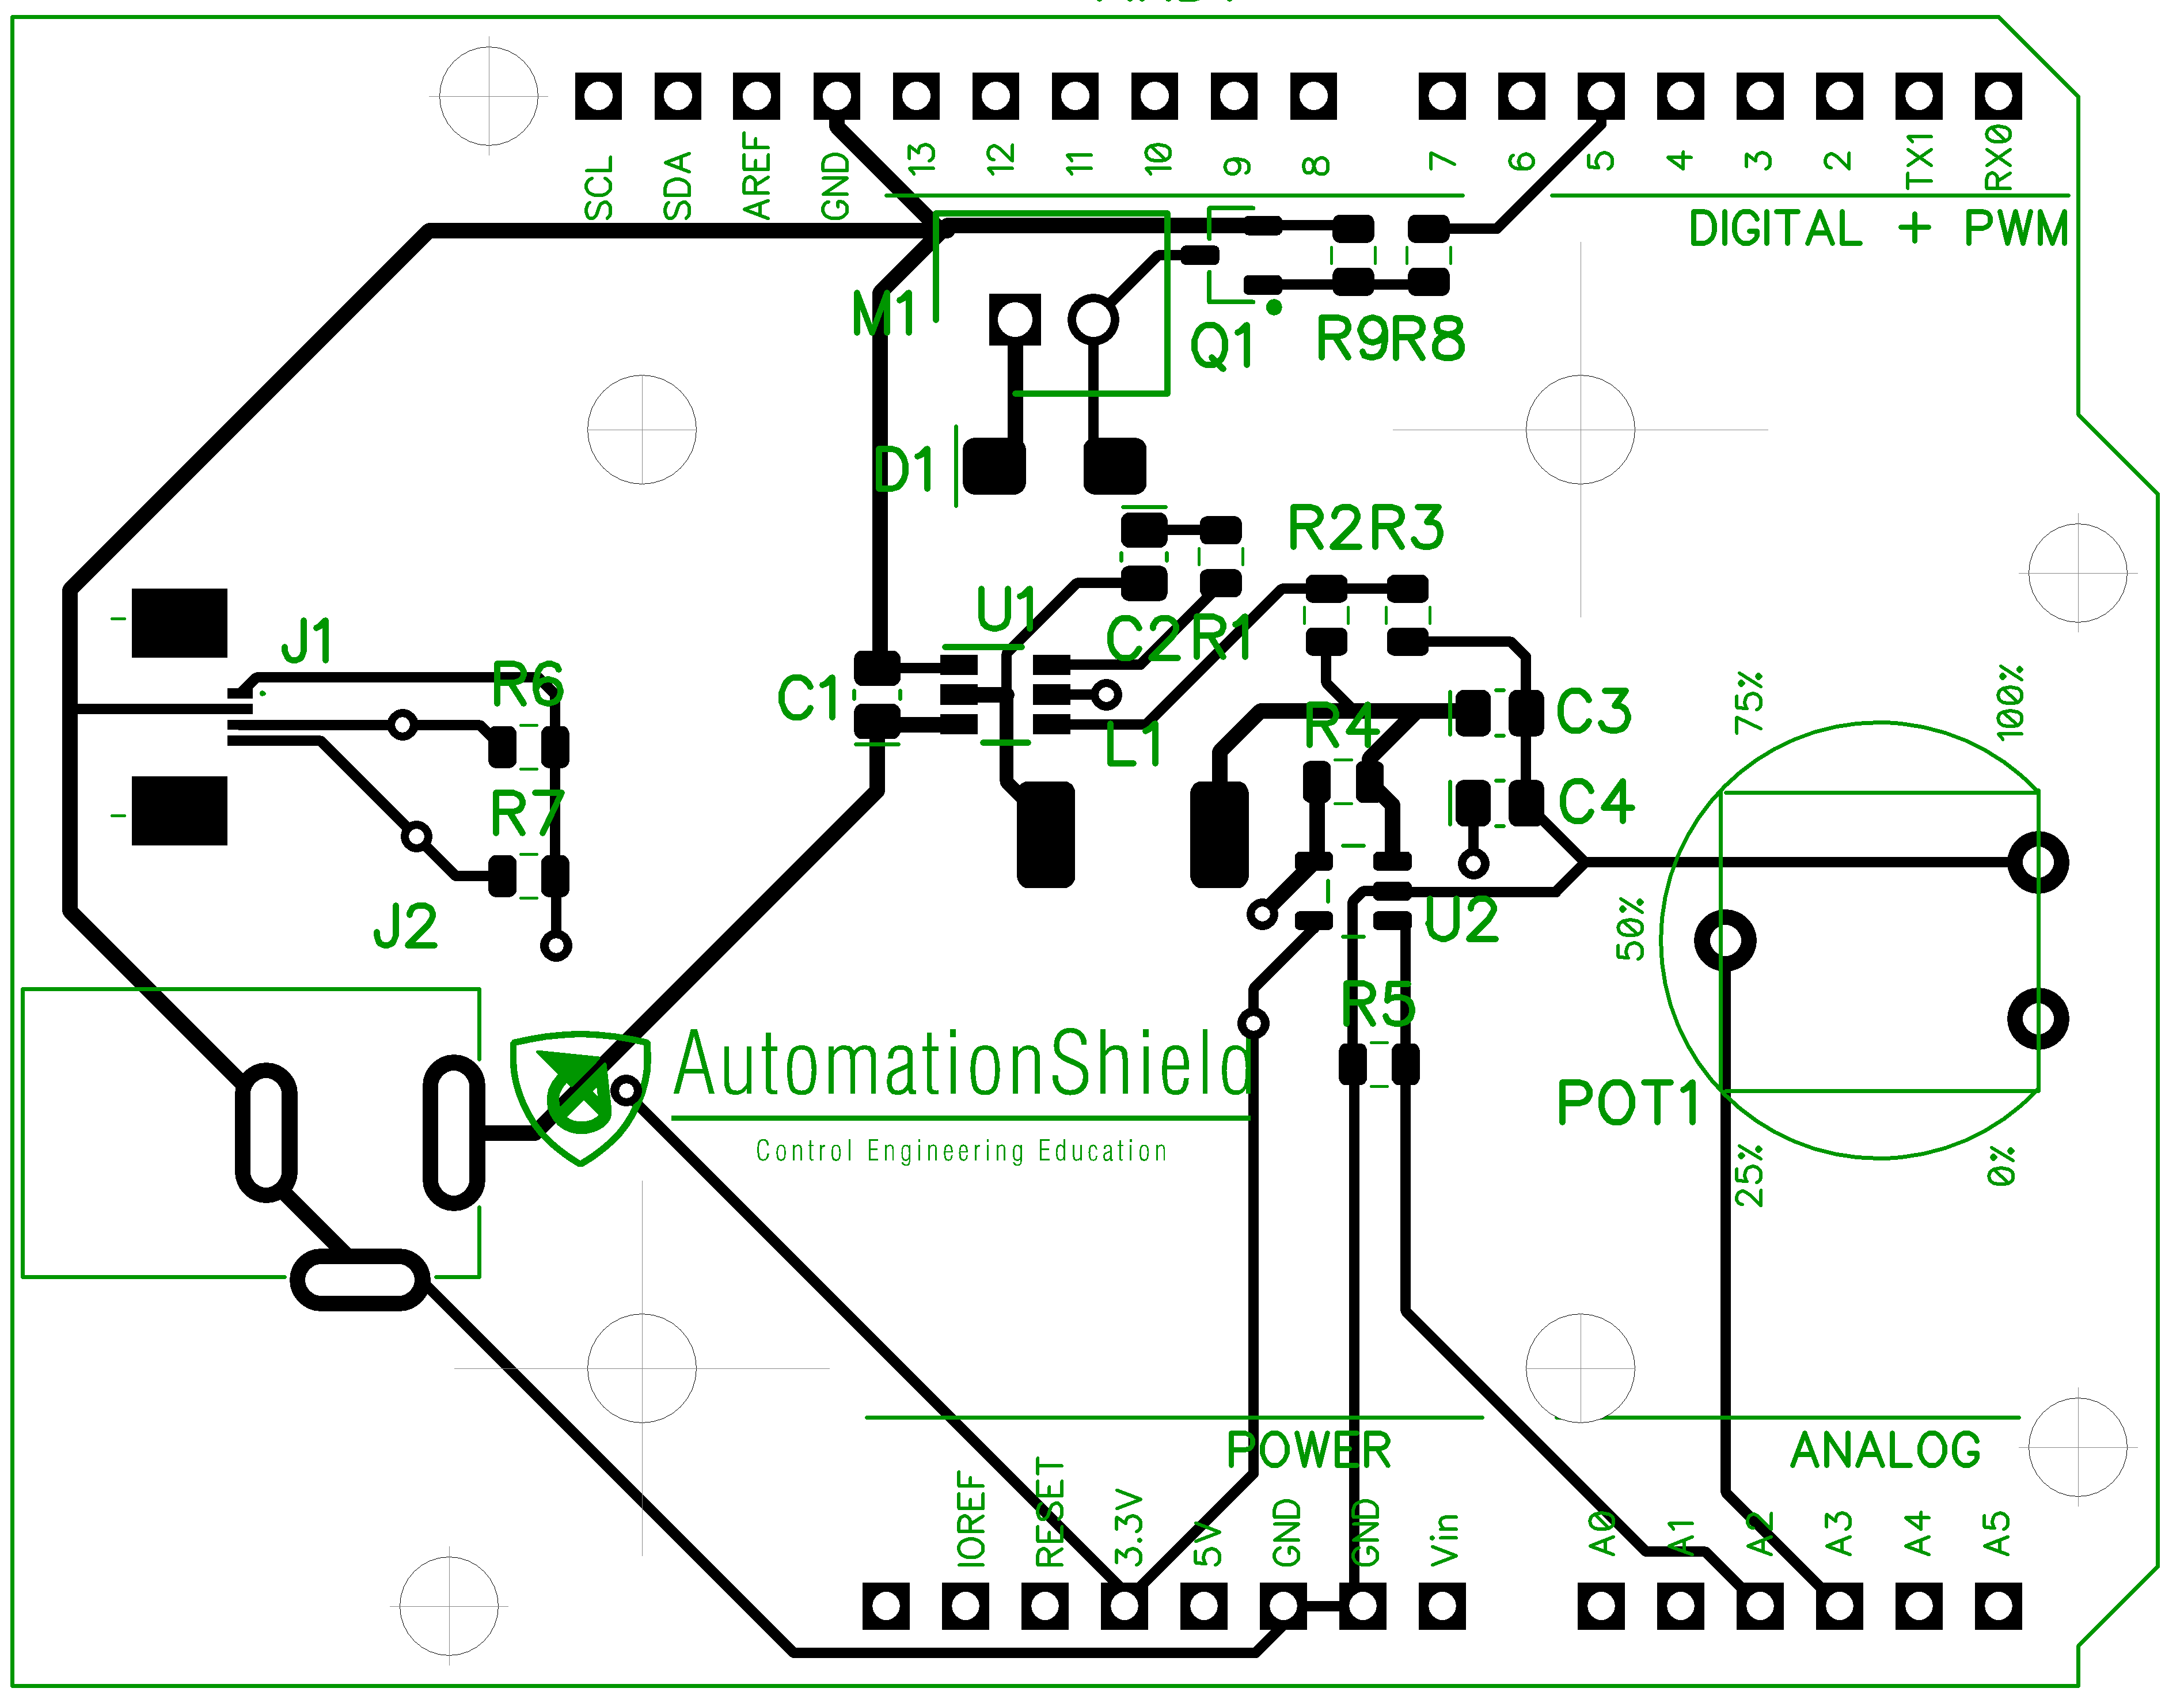
\includegraphics[width=8cm]{obr/AeroShieldTOP.png}

(a)

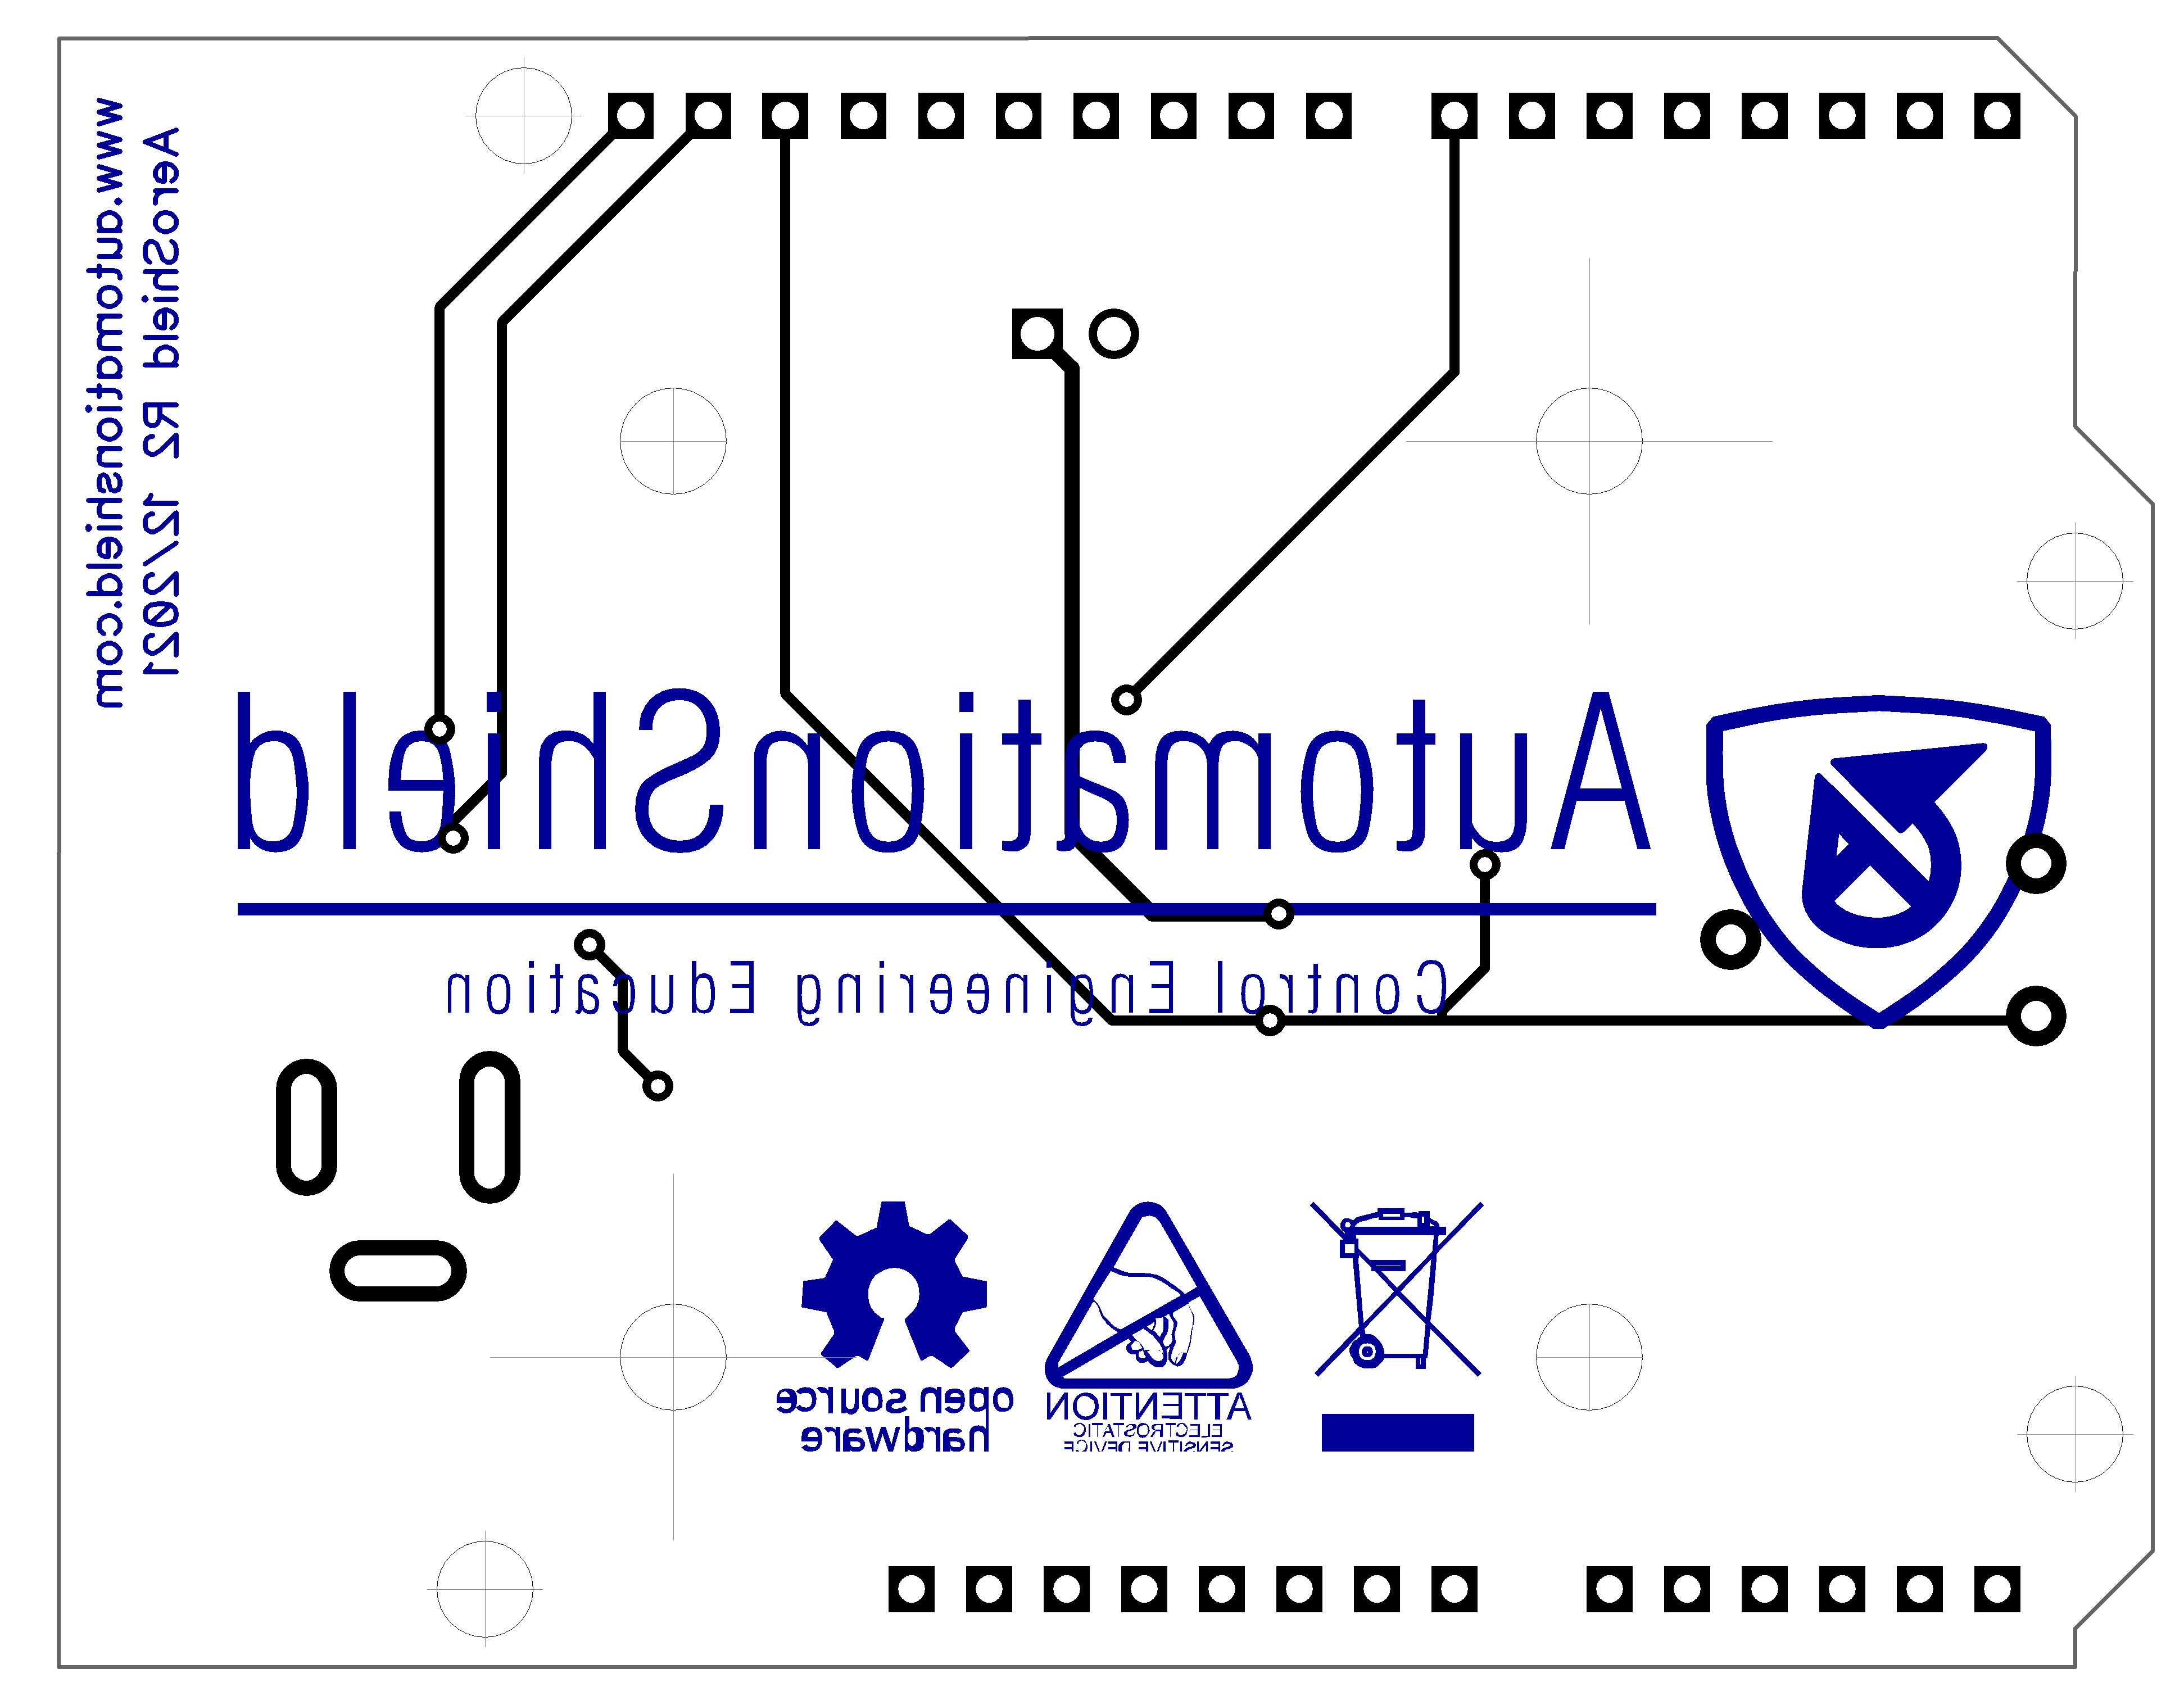
\includegraphics[width=8.5cm]{obr/AeroShieldBOTTOM.png}

(b)

\caption{(a) Vrchná strana AeroShieldu (b) Spodná strana AeroShieldu}
\label{OBRAZOK 2.4}
\end{figure}

\newpage

Po finálnej kontrole zapojenia komponentov na doske plošných spojov môžeme tieto dosky uložiť do formátu gerber. Súbory typu gerber v sebe ukladajú presné zloženie finálnej dosky plošných spojov a to po jej jednotlivých vrstvách. Nachádza sa tu teda vrstva zobrazujúca vodivé cesty, vrstva pre konektory via, vrstva pre farebné popisy a mnoho ďalších. Pri tvorbe súboru máme veľa možností aké parametre jednotlivých vrstiev chceme zvoliť. Môžeme meniť hrúbky jednotlivých vrstiev, veľkostí dier a priestoru okolo dier, veľkosti konektorov via a iné. Gerber súbor ďalej posielame výrobcovi PCB dosiek kde si môžeme zvoliť dalšie parametre dosky, ako jej farbu, možnosti pájkovacích doštičiek, dokonca nám môže výrobca poslať už napájkovanú dosku, ktorá je tak hneď pripravená na použitie. Podobu finálnej dosky AeroShieldu môžeme vidieť na obr.\ref{OBRAZOK 2.7}.a a dosky breakout boardu na obr.\ref{OBRAZOK 2.7}.b.


\begin{figure}[!tbh]
\hfill
\subfigure[Hlavná doska AeroShieldu]{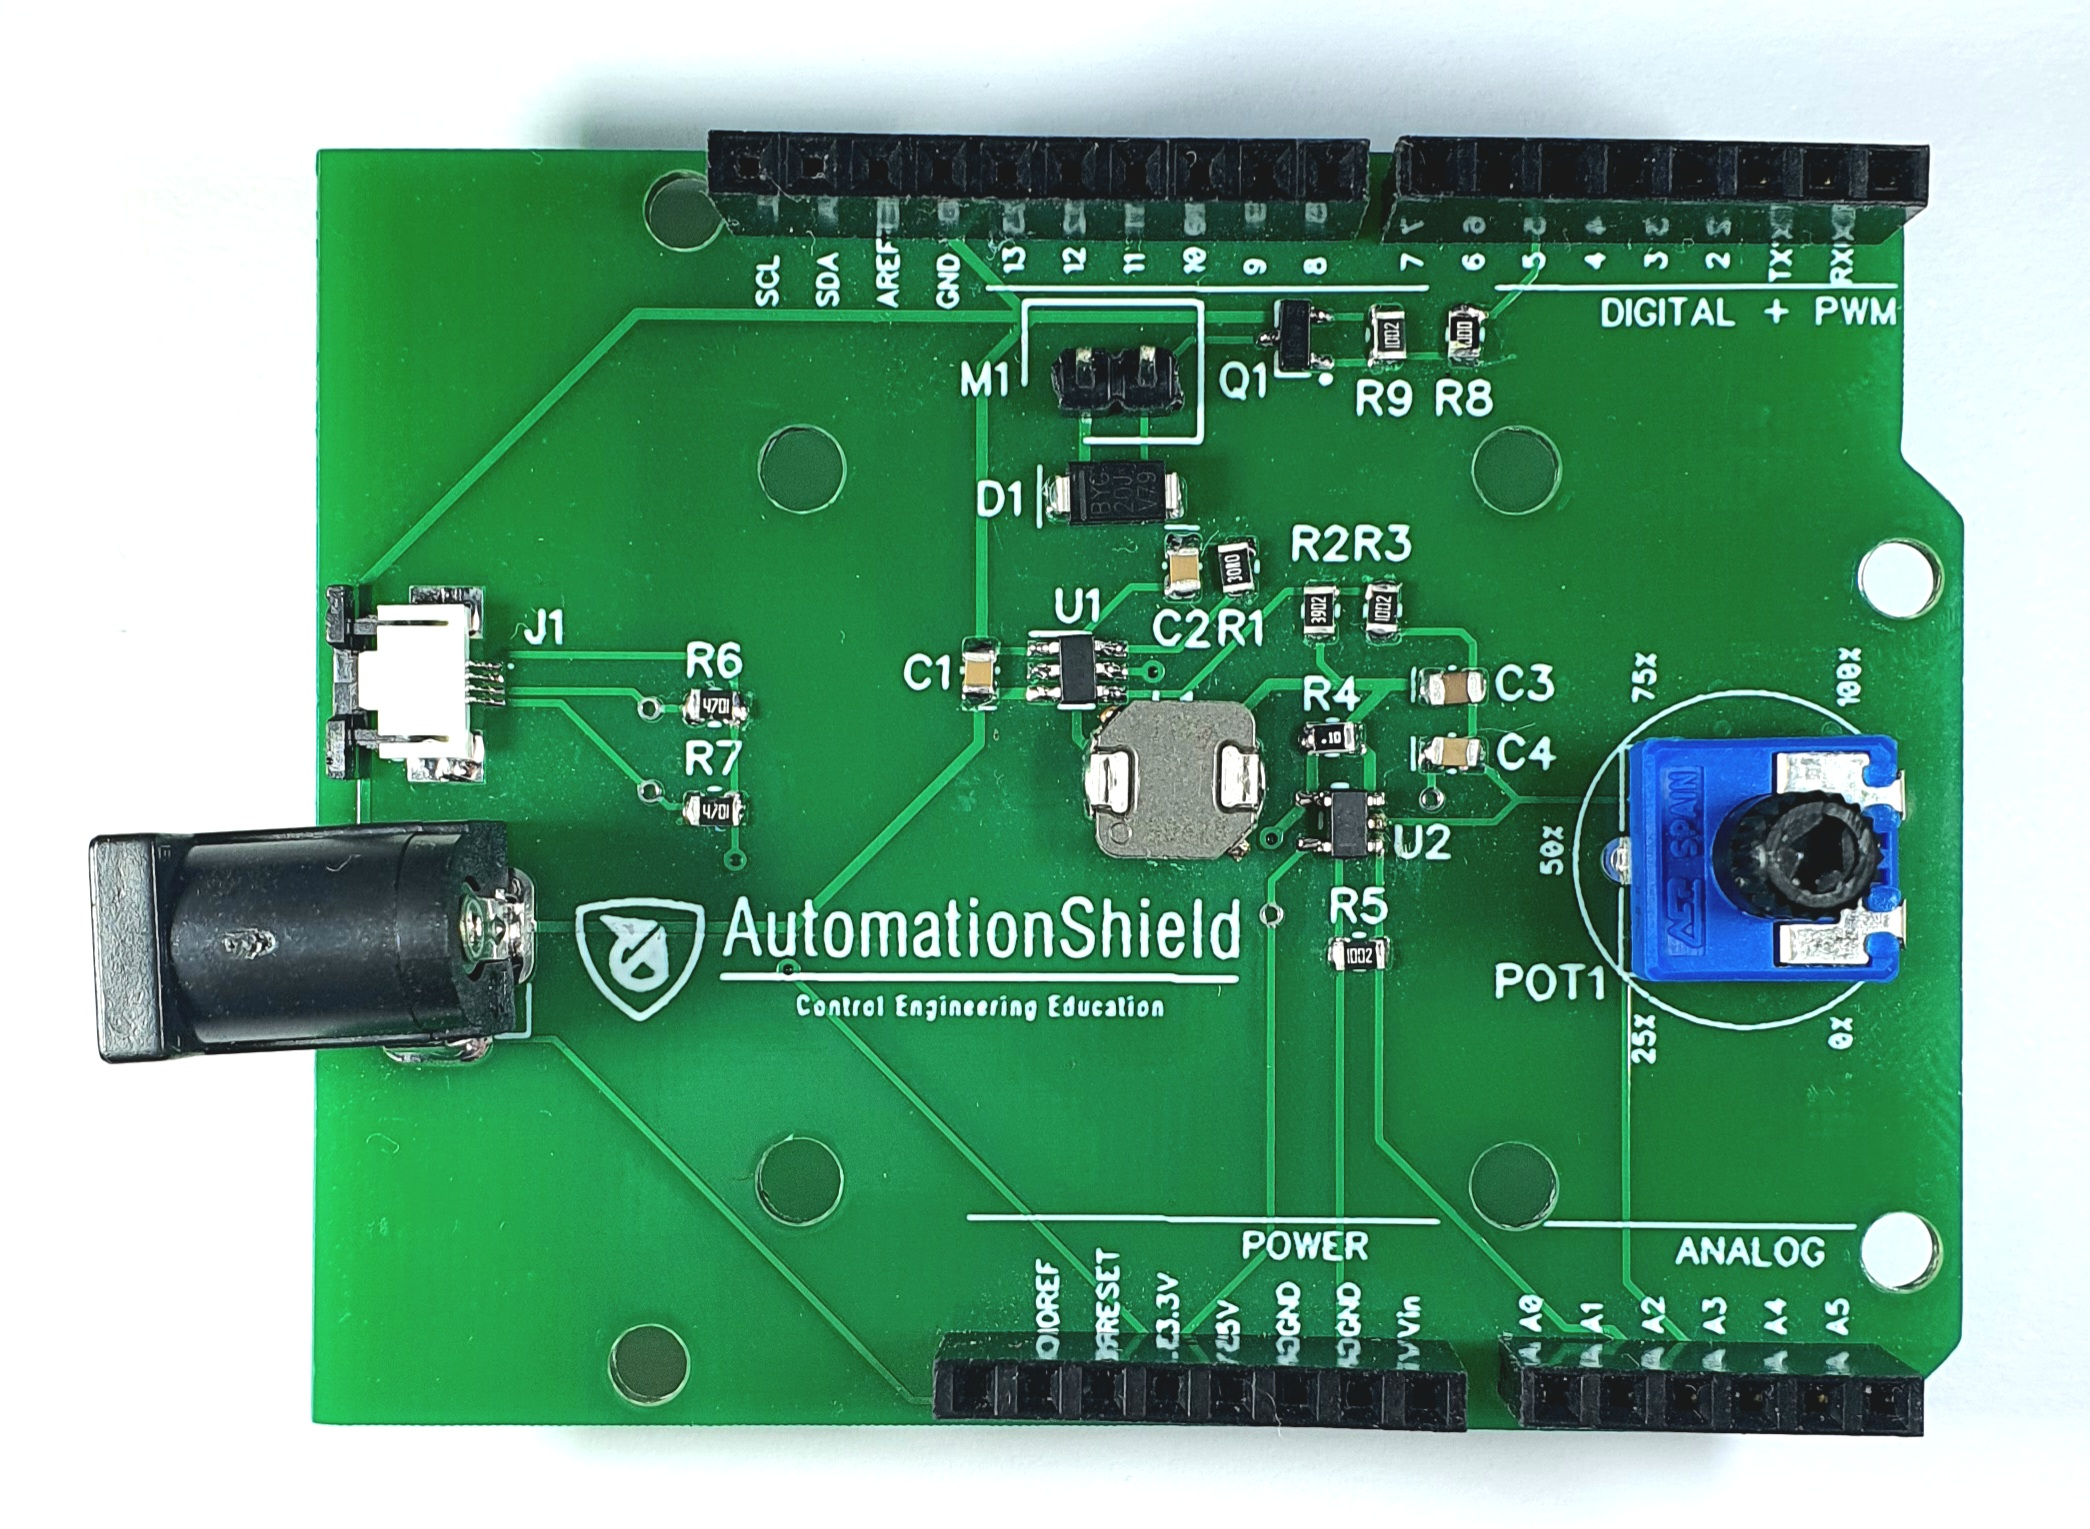
\includegraphics[width=9cm]{obr/AeroShield.jpg}}
\hfill
\subfigure[Vedľajšia doska AeroShieldu]{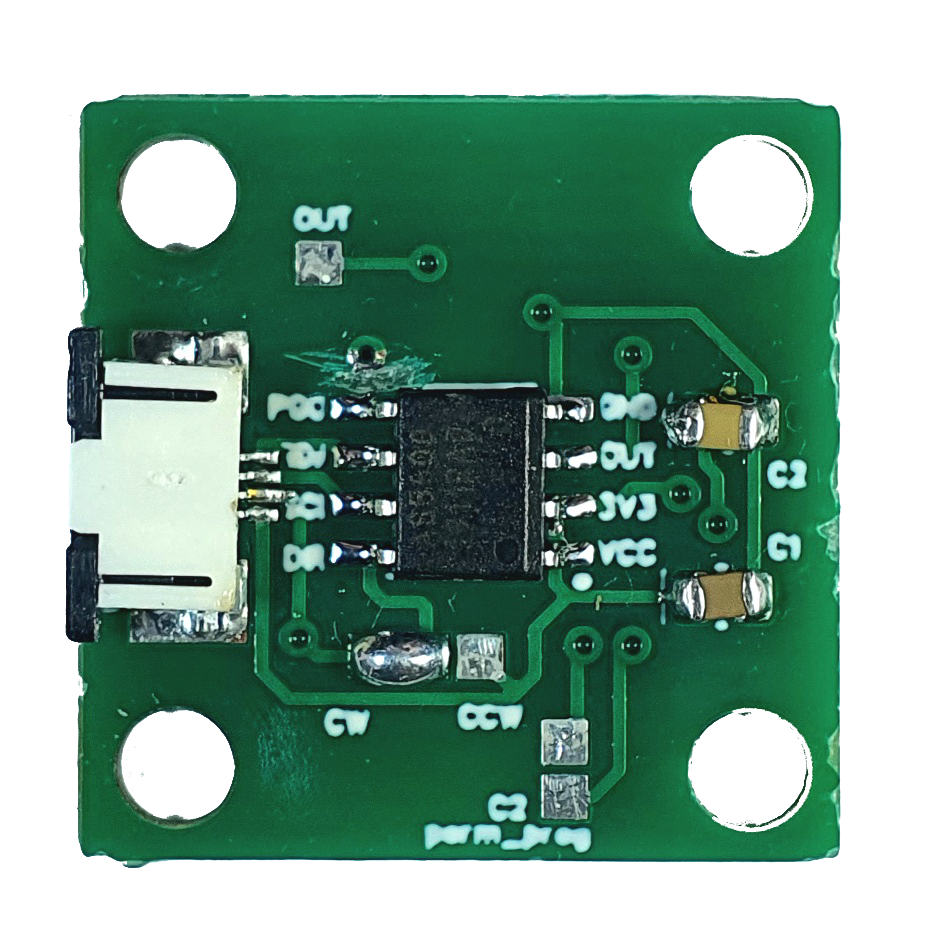
\includegraphics[width=6cm]{obr/fotoBreak.png}}
\hfill
\caption{Dosky plošných spojov AeroShieldu}\label{OBRAZOK 2.7}
\end{figure}


\section{Software}

Programovacie rozhranie pre platformy arduino sa nazýva Arduino IDE\footnote[5]{Arduino Integrated Development Environment.} a využíva programovací jazyk C++ resp. jeho podobu, s pridanými špecializovanými príkazmi a funkciami priamo pre arduino IDE. Príkazy sú na prvý pohľad zrozumiteľnejšie ako ich skompilovaná\footnote[6]{Kompilácia je preklad zdrojového kódu do podoby ktorú vie procesor prečítať a spracovať.} podoba v jazyku C++, no funkcie resp. schopnosti príkazu sú rovnaké. Preto je arduino vhodným prostriedkom na programovanie ako pre začiatočníkov, tak aj pre skúsenejších programátorov. 

Pri tvorbe programovej časti AeroShieldu je dôležité uvedomiť si fakt že doska vzniká v rámci projektu AutomationShield. Tým že je tento projekt opensource, ktokoľvek môže kód upravovať a vylepšovať, je preto dôležité aby funkcie navádzali používateľov na ich správne použitie a aby boli čo najviac prehľadné. Z tohoto dôvodu bola vytvorená knižnica AutomationShield ktorá v sebe zahŕňa najviac používané funkcie. Predstavme si situáciu kedy v programe ktorý píšeme potrebujeme premenu jednotiek z metrov na centimetre. Pokiaľ takúto funkciu použijeme v kóde jeden krát, môžeme túto funkciu napísať priamo do kódu. Avšak pokiaľ túto funkciu využívame častejšie, dáva zmysel uložiť ju mimo kód a následne túto funkciu zavolať naspäť v prípade jej potreby. Sprehľadňuje sa tak vzniknutý kód a znižuje sa možnosť chýb vďaka monotónnym kopírovaniam tej istej funkcie. 

Takúto možnosť externých preddefinovaných funkcií prístupných na zavolanie ponúka objektovo orientované programovanie(OOP) v jazyku C++\cite{oop}. Zvyčajne sa vytvárajú dva súbory resp. knižnice, z ktorých jedna sa nazýva \verb|headers| alebo hlavička s koncovkou .h a druhá, \verb|source| alebo zdrojový dokument s koncovkou .cpp. Header slúži ako akýsi navádzač a sklad pre premenné a funkcie, ktorý následne komunikuje so source dokumentom v ktorom sú uložené samotné funkcie. 

\subsection{Header}

Header súbor má niekoľko náležitostí ktoré obsahuje. Na začiatok deklarujeme súbor samotný. Robíme to pomocou príkazu \verb|#define|. Avšak, ak by sa takáto deklarácia nachádzala vo viacerých súboroch, a teda header súbor by sa načítal niekoľko krát, spôsobovalo by to problém pri kompilácii kódu. Z toho dôvodu používame funkciu \verb|Include guard| ktorá zamedzuje niekoľkonásobne načítanie rovnakých súborov. 

Hneď za definovaním knižnice AeroShild.h môžeme vkladať ďalšie knižnice, ktoré sú potrebné pre funkcie danej knižnice, a to pomocou príkazu \verb|#include|. Môžeme si všimnúť že za príkazom \verb|#include| sa nachádzajú dva typy zátvoriek resp. znakov. Konvencia je taká že na preddefinované knižnice sa používajú hranaté zátvorky \verb|<nazovKniznice.h>| a na knižnice tvorené programátormi sa používajú úvodzovky \verb|"nazovDalsejKniznice.h"|.

Za knižnicami následne určujeme premenné, ktoré majú priradené fyzické čísla pinov na arduine. Tieto premenné potom využívame buď na posielanie, alebo na prijímanie signálov z daných pinov. Názvy týchto premenných sa snažíme voliť tak, aby bola na prvý pohľad jasná ich funkcia, alebo podľa všeobecne zaužívaných pravidiel. V teórii riadenia sa na označenie vstupov používa písmeno \verb|R| a na označenie výstupov \verb|U,Y|. Príkaz \verb|#endif| vkladáme až na úplný záver header súboru.

\begin{lstlisting}[caption={Ukážka zdrojového kódu headeru.},captionpos=b]
#ifndef AEROSHIELD_H	 	 // Pokial nie je definovana AEROSHIELD_H
#define AEROSHIELD_H	 	 // Definuj kniznicu AEROSHIELD_H

#include "AutomationShield.h"    // Hlavna kniznica AutomationShieldu
#include <Wire.h>                // Kniznica potrebna pre komunikaciu I2C
#include <Arduino.h>		 // Zakladna arduino kniznica

#define AERO_RPIN A3             // Vstup z potenciometra
#define VOLTAGE_SENSOR_PIN A2    // Vstup pre meranie prudu 
#define AERO_UPIN 5              // Aktuator

----------------------Zdrojovy kod----------------------

#endif			   	 // Koniec if podmienky 
\end{lstlisting}



V časti \verb|Zdrojovy kod|, vytvárame \verb|class| alebo triedu ktorá v sebe zahŕňa funkcie a premenné ktoré sa nazývajú \verb|objects|, teda objekty. Class obsahuje podmnožinu objectov ktoré vieme prepájať a spájať vo väčšie celky, vďaka čomu vieme dosiahnuť veľmi komplexné funkcie. Tieto funkcie a premenné môžu byť buď \verb|public|, teda verejné a prístupné aj mimo súbor, alebo \verb|privat|, teda súkromné ktoré su prístupné len v knižniciach header a source. V header súbore sa môže nachádzať jedna, alebo viacero tried, záleží to od logicky deliteľných úsekov kódu, alebo od preferencie programátora. Deklarácia triedy s objektami vyzerá nasledovne: 

\begin{lstlisting}[caption={Triedy a objekty.},captionpos=b]
	class AeroShield{		// Deklaracia triedy
		public :		// Verejna cast
		void FirstObject();	// Deklaracia funkcie
		
		private :		// Sukromna cast
		float FirstVariable;	// Deklaracia premennej
	};				// Koniec triedy
\end{lstlisting}

V tomto prípade sa trieda nazýva AeroShield a má v sebe jednu funkciu s názvom \verb|FirstObject()| v časti public a jednu premennú \verb|FirstVariable|, typu float, v časti pivate. Rozdelenie na public a privat má zmysel hlavne v prípade ak chceme mať zadefinované isté premenné, pri ktorých nechceme aby sa dala externe zmeniť ich hodnota alebo typ. V prípade privat, takáto zmena nie je možná, jediná možnosť ako premennú zmeniť, je jej ručné prepísanie v súbore. V časti private deklarujeme funkcie ktoré následne využívame v rámci triedy a slúžia ako pomocné funkcie pri tvorbe komplexnejších častí kódu. V časti public sú funkcie viditeľné a schopné interagovať s inými triedami ako aj s inými knižnicami. 

\newpage
\subsection{Source}

Ako sme už spomínali, v knižnici source sa nachádzajú všetky funkcie využívané v AeroShielde. Keďže knižnice sa už definovali a načítavali v súbore header, stačí nám načítať len tento jeden súbor a to pomocou príkazu \code{#include "AeroShield.h"}, ktorý vložíme na začiatok súboru. Ďalej v súbore deklarujeme jednotlivé samostatné funkcie. Funkcie zapisujeme pomocou už spomínaného classu, dátového typu a názvu funkcie v podobe:
\begin{lstlisting}[caption={Source volanie funkcie.},captionpos=b]
typFunkcie AeroShield::nazovFunkcie()
\end{lstlisting}
V tomto prípade je AeroShield názov classu, nazovFunkcie hovorí sám za seba. Dátové typy funkcií poznáme rôzne. Vyberáme si ich na základe potreby ako chceme aby funkcia reagovala resp. aké hodnoty by mala prenášať. Dátové typy poznáme nasledovné\cite{datovetypy} (všetky hodnoty sú platné pre arduino UNO, pre iné typy arduina sa hodnoty môžu líšiť): 

\begin{table}[!ht]
	\centering
	\begin{tabular}{|p{0.22\textwidth} | p{0.22\textwidth} |p{0.22\textwidth} |p{0.22\textwidth} |}
		\hline
		\thead{dátový typ} & \thead{vlastnosti} & \thead{dátový typ} & \thead{vlastnosti} \\ \hline
		\textbf{array} & skupina premenných s priradeným indexom. Maximálna veľkosť je obmedzená veľkosťou pamäte RAM & \textbf{short }& 16 bitové celé čísla \\ \hline
		\textbf{boolean} & má buď hodnotu 0-nepravda, alebo 1-pravda & \textbf{char array }& spojenie viacerých dát typu char ukončené hodnotou null \\\hline
		\textbf{byte} & 8 bitové čísla od 0 do 255 & \textbf{string-object} & podobná funkcia ako object v header súbore \\ \hline
		\textbf{double} & rovnaké ako float & \textbf{unsigned char} & 8-bit znaky od 0 do 255 \\ \hline
		\textbf{float} & 32 bitové desatinne čísla $\pm$3.4028235E$+38$ & \textbf{unsigned int }& 16 bitové kladné celé čísla od 0 do 2$^{16}$-1 \\\hline
		\textbf{char} & 8 bit ascii tabulka & \textbf{unsigned long} & 32 bitové kladné celé čísla od 0 do 2$^{32}$-1 \\\hline
		\textbf{int} & 16 bitové celé čísla & \textbf{void }& nevracia naspäť žiadne informácie \\ \hline
		\textbf{long }& 32 bitové celé čísla & \textbf{word} & 16-bit číslo bez znamienka \\ \hline
    \end{tabular}
\caption{Dátové typy}
\label{tabulka typov}
\end{table}

\subsubsection{Popis použitých funkcií z knižnice AutomationShield}

Ako už bolo spomenuté, knižnica AutomationShield ponúka najviac používané funkcie, ktoré sa využívajú takmer na každom shielde. Pri rôznych veľkostiach a rozsahoch číselných stupníc, je dobré vyjadrovať hodnoty v percentách, namiesto ich absolútnej hodnoty. Arduino ponúka funkciu \verb|map()|, ktorá však pracuje len s dátovým typom integer. Aby sme docielili vyššiu presnosť, potrebujeme mapovať dátový typ float. Na tento účel nám slúži funkcia mapFloat do ktorej vstupuje veličina x, ktorej priradíme požadované hodnoty. Funkcie funguje na základe princípu lineárneho mapovania\cite{linearMap}.  

\begin{lstlisting}[caption={Zdrojový kód funkcie mapFloat.},captionpos=b]
float AutomationShieldClass::mapFloat(float x, float in_min, float in_max, float out_min, float out_max) 
{
return (x - in_min) * (out_max - out_min) / (in_max - in_min) + out_min; 
}
\end{lstlisting}

Ďalšou z funkcií použitých z knižnice AutomationShield je serialPrint. Funkcia vypisuje zvolený text na sériový monitor arduina. 

\begin{lstlisting}[caption={Zdrojový kód funkcie serialPrint.},captionpos=b]
 void AutomationShieldClass::serialPrint(const char *str){   
	#if ECHO_TO_SERIAL           // Pokial je tato funkcia povolena                       
	Serial.print(str);           // Vypis na seriovy monitor                       
	#endif 		// Koniec
}
\end{lstlisting}

\subsubsection{Popis použitých funkcií z knižnice AeroShield}


Keďže na AeroShielde využívame senzor hall efektu, musíme s ním v prvom rade nadviazať komunikáciu pomocou sériovej komunikácie I$^{2}$C. Protokol I$^{2}$C využíva na odosielanie a prijímanie údajov dva vodiče resp. dve linky: 
\begin{itemize}
\item sériovú dátovú linku (SDA-serial data), cez ktorú sa posielajú údaje, 
\item sériovú hodinovú linku (SCL-serial clock), na ktorú arduino v pravidelných intervaloch posiela impulzy. 
\end{itemize}

Hodinový pin udáva tempo komunikácie a je ovládaný mastrom. Mení stav v pravidelných impulzoch z low-nízkeho na high-vysoký stav. Pri každej takejto zmene je na dátový pin poslaný jeden bit informácie. Tieto bity najskôr obsahujú adresu zariadenia slave s ktorým chce master komunikovať, následne sa odosielajú bity príkazov. Keď sa táto informácia celá odošle, slave vykoná požiadavku a ak je to vyžadované, môže spätne mastrovi poslať údaje. Všetky tieto bity informácií sa posielajú na linke SDA\cite{idvac}.

I$^{2}$C funguje na princípe master-slave, kedy master je nadriadený a slave je podriadené zariadenie, s ktorým master komunikuje. Master môže naraz komunikovať s viacerými zariadeniami a to na základe jedinečných adries zariadení, ktoré sa medzi sebou striedajú v komunikácii.   

\subsubsection{Funkcia readOneByte()}

Pre naše účely postačuje vedieť čítať jeden alebo dva bajty informácií. Z toho dôvodu sme vytvorili dve funkcie: \code{int AeroShield::readOneByte()} a \newline\code{word AeroShield::readTwoBytes()}. Funkcia \code{int AeroShield::readOneByte()}, ako jej názov napovedá, získava 1 bajt informácii zo senzoru. Túto funkciu využívame napríklad na čítanie polohy kyvadla. 

\begin{lstlisting}[caption={Zdrojový kód funkcie readOneByte.},captionpos=b]
int AeroShield::readOneByte(int in_adr)         
{
	int retVal = -1;	 // Zadefinovanie pomocnej premennej
	Wire.beginTransmission(_ams5600_Address);// Zaciatok komunikacie 
	Wire.write(in_adr);	// Poziadavka na zaznamenianie uhlu kyvadla 
	Wire.endTransmission();	// Koniec komunikacie zo strany mastra
	Wire.requestFrom(_ams5600_Address, 1);	// Ziadost na odpoved  
	while (Wire.available() == 0);	// Cakaj pokial odpoved nepride  
	
	retVal = Wire.read();	// Zaznamenanie odpovede 
	
	return retVal;	// Zaslanie odpovede 
}
\end{lstlisting}

Ako môžeme vidieť v kóde funkcie, master najskôr osloví zariadenie slave, pomocou jeho adresy. Pri tomto konkrétnom čipe je adresa zariadenia v hexadecimálnej podobe 0x36. Následne zašle od výrobcu predprogramovanú žiadosť, ktorá zaznamená aktuálnu polohu magnetu resp. v našom prípade kyvadla. Následne je komunikácia ukončená a je zaslaná požiadavka na odpoveď zo strany slave zariadenia. Táto odpoveď je zaznamenaná a odoslaná späť, na miesto z ktorého bola funkcia privolaná.

\subsubsection{Funkcia readTwoBytes()}

Funkcia \code{word AeroShield::readTwoBytes()} je podobná predošlej funkcii, s rozdielom, že získané su dva bajty informácií narozdiel od jedného a na konci funkcie prebieha posun bitov\footnote[7]{Bitový posun je operácia vykonávaná so všetkými bitmi binárnej hodnoty, pri ktorej sa posúvajú o určený počet miest doľava alebo doprava\cite{biteShift}.}. 

\begin{lstlisting}[caption={Zdrojový kód funkcie readTwoBytes.},captionpos=b]
word AeroShield::readTwoBytes(int in_adr_hi, int in_adr_lo)        
{
	word retVal = -1;		// Zadefinovanie pomocnej premennej
	/* citanie "Low" bajtu */
	Wire.beginTransmission(_ams5600_Address);// Zaciatok komunikacie 
	Wire.write(in_adr);	// Poziadavka na zaznamenianie uhlu kyvadla 
	Wire.endTransmission();	// Koniec komunikacie zo strany mastra
	Wire.requestFrom(_ams5600_Address, 1);	// Ziadost na odpoved  
	while (Wire.available() == 0);	// Cakaj pokial odpoved nepride  

	int low = Wire.read();     	// Ulozenie prveho bajtu 
	/* citanie "High" bajtu */
	Wire.beginTransmission(_ams5600_Address);// Zaciatok komunikacie 
	Wire.write(in_adr);	// Poziadavka na zaznamenianie uhlu kyvadla 
	Wire.endTransmission();	// Koniec komunikacie zo strany mastra
	Wire.requestFrom(_ams5600_Address, 1);	// Ziadost na odpoved  
	while (Wire.available() == 0);	// Cakaj pokial odpoved nepride  
	
	word high = Wire.read();   	// Ulozenie druheho bajtu 
	
	high = high << 8;          	// Posun bitov
	retVal = high | low;
	
	return retVal;	   	  	// Zaslanie odpovede 
}
\end{lstlisting}

\subsubsection{Funkcia detectMagnet()}

Ďalšou dôležitou funkciou, je zistiť prítomnosť magnetu na kyvadle. Túto úlohu vykonáva funkcia \code{int AeroShield::detectMagnet()}. Využívame ju vždy pri inicializácii AeroShieldu, na to aby sme zistili či nenastali problémy s magnetom, alebo so senzorom samotným. Funkcia komunikuje so senzorom, a na základe výstupu vieme určiť či bol magnet detegovaný. Funkcia nám vráti na výstupe 1- pokiaľ sa magnet nachádza pri senzore a 0- pokiaľ magnet nie je prítomný, alebo je príliš vzdialený od senzoru. 

\begin{lstlisting}[caption={Zdrojový kód funkcie detectMagnet.},captionpos=b]
int AeroShield::detectMagnet() 
{
	int magStatus;		// Pomocna premenna  
	int retVal = 0;		// Pomocna premenna
	magStatus = readOneByte(_stat);	// Prebieha komunikacia so senzorom                        
	
	if (magStatus & 0x20)		// Pokial je podmeinka splnena vrat 1, pokial nie je splnena vrat 0 
	retVal = 1;
	
	return retVal;			// Zaslanie odpovede 
}
\end{lstlisting}

\subsubsection{Funkcia getMagnetStrength()}

Pre správnosť fungovania hall senzoru je dôležité dodržať správnu vzdialenosť magnetu od senzoru. Výrobca udáva že najideálnejšia vzdialenosť je 0.5-3mm, v závislosti na sile a veľkosti magnetu. Bolo by nepraktické túto vzdialenosť merať ručne, použijeme preto funkciu \code{int AeroShield::getMagnetStrength()}. Môžeme si všimnúť že táto funkcia používa rovnaký príkaz na komunikáciu so senzorom, ako aj funkcia \code{detectMagnet()} a to síce \verb|_stat|. Z toho vyplýva že \code{detectMagnet()} kontroluje nielen prítomnosť magnetu, ale aj jeho správnu vzdialenosť. Pokiaľ teda dostaneme z funkcie \code{detectMagnet()} ako výsledok 1, vieme že magnet je prítomný a zároveň v ideálnej vzdialenosti. Funkcia \code{getMagnetStrength()} je teda iba doplňujúcou funkciou, ktorá nám určí či je magnet moc blízko senzoru, výsledná hodnota výstupu bude 3, alebo naopak, je magnet moc vzdialený a výstupná hodnota bude 1. 

\begin{lstlisting}[caption={Zdrojový kód funkcie getMagnetStrength.},captionpos=b]
int AeroShield::getMagnetStrength()   
{
	int magStatus;                  // Pomocna premenna 
	int retVal = 0;                 // Pomocna premenna
	magStatus = readOneByte(_stat);	// Prebieha komunikacia so senzorom       
	
	if (detectMagnet() == 1)	// Pokial je splnena podmienka detectMagnet()
	{
		retVal = 2;  // Vrat 2, magnet je v idelnej vzdialenosti
		if (magStatus & 0x10)
		retVal = 1;  // Vrat 1, magnet je v prilis daleko
		else if (magStatus & 0x08)
		retVal = 3;  // Vrat 3, magnet je v prilis blizko
	}
	
	return retVal;                  // Zaslanie odpovede  
}
\end{lstlisting}

\subsubsection{Funkcia getRawAngle()}

Poslednou funkciu komunikácie s hall senzorom je \code{word AeroShield::getRawAngle()}. Funkcia slúži na čítanie samotného uhlu kyvadla. Výsledkom tejto funkcie je číslo s rozsahom 12bitov, teda číslo od 0 do 4096 ktoré udáva momentálnu polohu kyvadla. O tomto senzore, ako aj o jeho fungovaní sme už hovorili bližšie v časti \ref{meruhl}. 

\begin{lstlisting}[caption={Zdrojový kód funkcie getRawAngle.},captionpos=b]
word AeroShield::getRawAngle() 
{
	return readTwoBytes(_raw_ang_hi, _raw_ang_lo); // Prebieha komunikacia so senzorom, ktory rovno vrati vysledok pomocou prikazu return 
}
\end{lstlisting}

\subsubsection{Funkcia begin()}

Prvou z funkcií mimo komunikácie s hall senzorom je \code{float AeroShield::begin(bool isDetected)}, do ktorej vstupuje výsledok z funkcie \code{detectMagnet()} ako premenná \verb|isDetected|. Funkcia \code{begin()} nastaví pin potrebný na ovládanie akčného člena, pomocou príkazu \verb|pinMode|, ako výstup, teda \verb|OUTPUT|. Zároveň inicializuje sériovú komunikáciu I$^{2}$C. Príkaz na započatie komunikácie I$^{2}$C sa pri rôznych typoch dosiek, resp. architektúr mikroradiča Arduino líši. Použijeme preto podmienku \verb|#ifdef| za ktorou nasleduje typ architektúry daného mikroradiča a príslušný príkaz pre začiatok sériovej komunikácie I$^{2}$C. V prípade Arduino UNO, je to príkaz \verb|Wire.begin()|. 

Zároveň je vo funkcii \code{begin()}, pomocou if podmienky, kontrolovaná premenná \verb|isDetected|. Pokiaľ bol magnet detegovaný, vypíše na sériový port správu "Magnet detected$"$ a while\footnote[8]{Cyklus while sa bude opakovať nepretržite, pokiaľ sa výraz vnútri zátvoriek () nestane nepravdivým.} cyklus, sa pomocou príkazu \verb|break| ukončí. Pokiaľ magnet detegovaný nebol, vypíše "Can not detect magnet", no while cyklus pokračuje.  


\begin{lstlisting}[caption={Zdrojový kód funkcie begin.},captionpos=b]
float AeroShield::begin(bool isDetected){ 
	pinMode(AERO_UPIN,OUTPUT);	// Pin aktuatora
	
	#ifdef ARDUINO_ARCH_AVR		// Pre dosky s architekturov AVR
	Wire.begin();			// Pouzi objekt Wire
	#elif ARDUINO_ARCH_SAM      	// Pre dosky s architekturov SAM
	Wire1.begin();			// Pouzi objekt Wire1
	#elif ARDUINO_ARCH_SAMD     	// Pre dosky s architekturov SAMD
	Wire.begin();			// Pouzi objekt Wire
	#endif
	
	if(isDetected == 0 ){       	// Pokial magnet nie je detegovany
		while(1){               // While podmienka
		 if(isDetected == 1 ){	// Pokial sa magnet deteguje
		  AutomationShield.serialPrint("Magnet detected \n");	
		break;		    // Koniec while podmienky
		}
		else{               // Pokial magnet nie je detegovany
		  AutomationShield.serialPrint("Can not detect magnet \n");
			}
		}
	}       
} 
\end{lstlisting}

\subsubsection{Funkcia calibration()}

Ďalšou v poradí je funkcia \code{calibration()}. Slúži na prepočet a zaznamenanie nulovej polohy kyvadla, teda takej polohy v ktorej sa kyvadlo nachádza, pokiaľ motorček nie je poháňaný. V ideálnom prípade by sa kyvadlo vždy po vypnutí motora vrátilo do rovnakej východzej polohy. Avšak kyvadlo je prepojené s motorom a shieldom pomocou káblov, ktoré tvoria odpor a teda kyvadlo sa vždy zastaví v inej nulovej polohe. Funkcia \code{calibration()} teda slúži na zaznamenanie tejto nulovej polohy a všetky následné výpočty sa odvolávajú práve na túto hodnotu. 

Do funkcie vstupuje hodnota aktuálneho uhlu kyvadla, z funkcie \code{getRawAngle()} ako premenná \verb|RawAngle|. Funkcia na začiatok vypíše text "Calibration running..." a motorček zapneme na štvrť sekundy na výkon 20\%. Kyvadlo sa začne kývať a počkáme štyri sekundy, pokiaľ sa ustáli. Keď je kyvadlo ustálené zaznamenáme jeho hodnotu do premennej \verb|startangle|. Následne prebieha for cyklus ktorý zvukovo informuje o dokončenej kalibrácii pomocou troch pípnutí. Využívame tu jav, pri ktorom motorček vydáva vysoký tón, pokiaľ je do neho privádzaný nízky PWM signál. 

\begin{lstlisting}[caption={Zdrojový kód funkcie calibration.},captionpos=b]
float AeroShield::calibration(word RawAngle) {  
	AutomationShield.serialPrint("Calibration running...\n");  
	startangle=0;              // Vynulovanie premennej 
	analogWrite(AERO_UPIN,50); // Spustenie motora na vykon 20%
	delay(250);                // Cakaj 0.25s 
	analogWrite(AERO_UPIN,0);  // Vypnutie motora
	delay(4000);               // Cakaj 4s
	
	startangle = RawAngle;     // Uloz hodnotu nuloveho uhla
	analogWrite(AERO_UPIN,0);  // Poistne vypnutie motora 
	for(int i=0;i<3;i++){      // Funkcia na zvukovu signalizaciu
		analogWrite(AERO_UPIN,1);     // Zapnutie motora
		delay(200);                   // Cakaj
		analogWrite(AERO_UPIN,0);     // Vypnutie motora
		delay(200);                   // Cakaj
	}
	
	AutomationShield.serialPrint("Calibration done");
	return startangle;                    // Vrat hodnotu 
}
\end{lstlisting}

\subsubsection{Funkcia convertRawAngleToDegrees()}

Ako sme už spomínali v sekcii \ref{meruhl}, zaznamenávaná hodnota uhlu kyvadla je v rozmedzí od 0 do 4096 a tieto hodnoty priamo korešpondujú zo stupňami od 0\textdegree  do 360\textdegree. 1\textdegree  predstavuje hodnotu približne 11.77 vo formáte raw. Funkcia \code{convertRawAngleToDegrees()} teda len zoberie raw hodnotu uhlu a vynásobí ju hodnotou $\dfrac{360\textdegree}{4096}$ =0.087\textdegree. Funkcia teda naspäť vráti prepočítanú hodnotu uhla kyvadla v stupňoch. 

\begin{lstlisting}[caption={Zdrojový kód funkcie convertRawAngleToDegrees.},captionpos=b]
float AeroShield::convertRawAngleToDegrees(word newAngle) {  
	float ang = newAngle * 0.087;    // 360/4096=0.087 x rawHodnota                             
	return ang;                      // Vrat hodnotu
}
\end{lstlisting}


\subsubsection{Funkcia referenceRead()}

Funkcia \code{referenceRead()} slúži na čítanie hodnoty z potenciometra, ktorý sa nachádza na shielde, a jeho následne premapovanie do percentuálnej podoby. Potenciometer využívame na manuálne ovládanie AeroShieldu a v ďalších funkciách, sa využíva hlavne jeho percentuálna hodnota. Vrátená hodnota je typu float, v škále od 0.0\% do 100.0\%. 

\begin{lstlisting}[caption={Zdrojový kód funkcie referenceRead.},captionpos=b]
	  float AeroShield::referenceRead(void) {      
		referencePercent = AutomationShield.mapFloat(analogRead(AERO_RPIN), 0.0, 1024.0, 0.0, 100.0);  
		 // Premapovanie originalnej hodnoty 0.0-1023 na percentualny rozsah 0.0-100.0
		return referencePercent;      // Vrat percentualnu hodnotu 
	}
\end{lstlisting}
	
\subsubsection{Funkcia actuatorWrite()}	
	
Na ovládanie motora resp. jeho otáčok, používame funkciu \code{actuatorWrite()}. Do funkcie vstupuje percentuálna hodnota výkonu motora, táto hodnota je premapovaná na PWM signál, potrebný na správne ovládanie motora. Tento signál následne vstupuje do ochrannej funkcie \code{constrainFloat()}, ktorá zabezpečí aby sa hodnota PWM signálu mohla pohybovať len v rozmedzí od 0.0 do 255.0. Táto hodnota je potom zapísaná na príslušný pin motora, v našom prípade je to \verb|AERO_UPIN|. 
	
	
\begin{lstlisting}[caption={Zdrojový kód funkcie actuatorWrite.},captionpos=b]
	void AeroShield::actuatorWrite(float PotPercent) {   
		float mappedValue = AutomationShield.mapFloat(PotPercent, 0.0, 100.0, 0.0, 255.0);       
		// Vstupna percentualna hodnota 0.0-100.0 premapovana na hodnoty 0.0-255.0
		mappedValue = AutomationShield.constrainFloat(mappedValue, 0.0, 255.0);  
		// Bezpecnostna funkcia obmedzenia premapovanej hodnoty
		analogWrite(AERO_UPIN, (int)mappedValue);  // Zapisanie hodnoty na pin
	}
\end{lstlisting}
	
	
\subsubsection{Funkcia currentMeasure()}	
	
Poslednou funkciou AeroShieldu je \code{currentMeasure()}. Funkcia slúži na zaznamenávanie prúdu, ktorý odoberá motor kyvadla. Fungovanie snímača je opísané v sekcii \ref{merprud}. Funkcia slúži na prepočítanie zaznamenanej hodnoty napätia na prúd. Funkcia beží vo for cykle, ktorý sa opakuje \verb|repeatTimes|-krát, z dôvodu presnejšieho merania, keďže meraná hodnota sa priveľa mení, čo skresľuje výslednú hodnotu. Vďaka for cyklu získame priemernú hodnotu prúdu. 

Výsledná hodnota prídu prechádza úpravami, pomocou dvoch korekčných premenných, ktoré sme získali vďaka meraniam prúdu pomocou multimetra, a následným porovnaním hodnôt zo senzora. Porovnaním hodnôt sme získali veľkosti korekčných premenných, vďaka čomu sa naše merania zhodujú s meraniami pomocou multimetra, na dve desatinné miesta. 

Prevod z napätia na prúd robíme podľa pokynov uvedených v zdrojovom dokumente senzoru. Pri tomto prevode využívame hodnotu shunt rezistora \verb|RS|, ako aj hodnotu rezistora \verb|RL|, ktorý priamo premieňa prúd na napätie. 

Kedže prúd nemôže vykazovať záporné hodnoty(iba pokiaľ prúdi opačným smerom, ako sme zamýšľali), na záver funkcie ešte prechádza if podmienkou, ktorá zmení záporné hodnoty prúdu na hodnotu 0.000A.  
	
\begin{lstlisting}[caption={Zdrojový kód funkcie currentMeasure.},captionpos=b]	
float AeroShield::currentMeasure(void){  
	for(int i=0 ; i<repeatTimes ; i++){     // For cyklus
	voltageValue= analogRead(VOLTAGE_SENSOR_PIN);     
	// Citanie hodnoty zo senzoru INA169 
	voltageValue= (voltageValue * voltageReference) / 1024;    
	// Mapovanie hodnoty zo senzoru, na realnu hodnotu napatia(referencne napatie je 5V)
	current= current + correction1-(voltageValue / (10 * ShuntRes));    
                // Vzorec na vypocet prudu
                // Is = (Vout x 1k) / (RS x RL)
}                                                                         	
	float currentMean= current/repeatTimes;   
	// Vypocet priemernej hodnoty  
	currentMean= currentMean-correction2;       // Korekcia
	if(currentMean < 0.000) currentMean= 0.000;                 
	                    // Korekcia nulovej hodnoty
	current= 0;         // Vynulovanie pomocnych premennych   
	voltageValue= 0;    // Vynulovanie pomocnych premennych   
	return currentMean; // Vrat hodnotu prudu v amperoch
}
\end{lstlisting}
	
	
	
	
	
	
píš aj o samplingu  

\chapter{Didaktické príklady}

Pre AeroShield bolo v prostredí Arduino IDE, MATLAB a Simulink vytvorených niekoľko vzorových programov, ktoré demonštrujú všetky jeho funkcie a možnosti operácie. Programy sú rozdelené do dvoch veľkých skupín, konkrétne programy v otvorenej slučke bez spätnej väzby a programy v uzavretej slučke so spätnou väzbou. 

Ich rozdiel spočíva v tom že pri riadení bez spätnej väzby, hovoríme o ovládaní systému, kedy sa snažíme dosiahnuť žiadané hodnoty výstupov bez spätnej informácie o vykonaní procesu, alebo o jeho hodnote. V prípade riadenia so spätnou väzbou sa jedná o reguláciu. Pri regulácii sa kontroluje bezprostredný účinok riadenia, ktorý sa porovnáva so žiadanou hodnotou výstupu a na vyrovnanie ich vzájomnej chyby, sa okamžite vykonáva zásah do vstupných veličín. 

\section{Programy v otvorenej slučke, bez spätnej väzby}
\subsection{$AeroShield_OpenLoop.ino$}

Ako prvý príklad si ukážeme program s názvom \verb|AeroShield_OpenLoop.ino| napísaný v prostredí Arduino IDE. Hlavnou ideou tohoto programu je jednoduché ovládanie otáčok motorčeka kyvadla, pomocou potenciometra. Na začiatku programu inicializujeme hlavnú knižnicu AeroShieldu pomocou príkazu \verb|#include "AeroShield.h"|. Následne deklarujeme premenné, ktorých hodnoty budú vypisované na sériový monitor. 

\begin{lstlisting}[caption={AeroShield open loop dekleracia.},captionpos=b]
#include "AeroShield.h"       //  Inicializacia hlavnej kniznice

float startangle=0;           //  Premenna pre nulovy uhol
float lastangle=0;            //  Premenna pre maximalny uhol 
float pendulumAngle;          //  Uhol natocenia kyvadla
float referencePercent;       //  Hodnota potenciometra
float CurrentMean;	      //  Hodnota prudu odoberaneho motorom 
\end{lstlisting}

Nasleduje časť \verb|setup()|, v ktorej ako prvé, prebehne nastavenie rýchlosti sériovej komunikácie \verb|Serial.begin(115200)|. Číslo 115 200 predstavuje počet zmien, stavu z 0 na 1 resp. zo stavu high na stav low, za sekundu. Nasleduje funkcia \verb|AeroShield.begin()| ktorá sleduje prítomnosť magnetu, a pred nastaví potrebné premenné a funkcie pinov. Poslednou funkciou je kalibrácia kyvadla \verb|AeroShield.calibration()|, spolu s výpočtom začiatočného a koncového uhla. 

\begin{lstlisting}[caption={AeroShield open loop setup().},captionpos=b]
void setup() {                // Setup prebehne len jeden krat 
 Serial.begin(115200);       // Zaciatok seriovej komunikacie 
 AeroShield.begin(AeroShield.detectMagnet());  // Inicializacia AeroShieldu 
 startangle = AeroShield.calibration(AeroShield.getRawAngle());   // Kalibracia kyvadla
 lastangle=startangle+1024;  // Kalkulacia uhlu kyvadla pre map function
}
\end{lstlisting}

V časti \verb|loop()| sa program opakuje dookola. Ako prvé, prebehne mapovanie uhlu kyvadla pomocou funkcie \verb|AutomationShield.mapFloat()| a získaná hodnota uhlu sa vypíše na sériový monitor, spolu s názvom a premennou danej veličiny. Nasleduje čítanie hodnoty potenciometra, ktorá slúži na ovládanie akčného člena pomocou funkcie \verb|AeroShield.actuatorWrite()|. Na sériový port sa vypíše hodnota potenciometra, za ktorou nasleduje veľkosť prúdu odoberaného motorom \verb| AeroShield.currentMeasure()|. 

\begin{lstlisting}[caption={AeroShield open loop loop().},captionpos=b]
void loop() {
	pendulumAngle= AutomationShield.mapFloat(AeroShield.getRawAngle(),startangle,lastangle,0.00,90.00);    //  Mapovanie uhlu kyvadla 
	Serial.print("pendulum angle is: ");
	Serial.print(pendulumAngle);    
	Serial.print("\textdegree || ");
	
	referencePercent= AeroShield.referenceRead();  // Citanie potenciometra
	Serial.print("pot value is: ");
	Serial.print(referencePercent);  
	Serial.print("% || ");
	
	AeroShield.actuatorWrite(referencePercent); // Pohyb akcneho clenu
	
	CurrentMean= AeroShield.currentMeasure();  // Meranie prudu
	Serial.print("current value is: ");
	Serial.print(CurrentMean);   
	Serial.println("A || ");
}
\end{lstlisting}

\subsection{$AeroShield_Open_Loop.m$}


\section{Programy v uzatvorenej slučke, so spätnou väzbou}

sampling aj
\chapter{Záver}

Táto časť diplomovej práce je povinná. Autor práce uvedie zhodnotenie riešenia, jeho výhody resp. nevýhody, použitie výsledkov, ďalšie možnosti a podobne.  Môže aj načrtnúť iný spôsob riešenia úloh, resp. uvedie, prečo postupoval uvedeným spôsobom.

%\chapter{Základné triky v LaTeX}
\label{jablka}

% Toto je komentár

Úloha tejto kapitoly je poukázať na niektoré základné triky v LaTeX pri písaní záverečnej práci. Vygenerované PDF-čko spolu so zdrojovým kódom by mali slúžiť ako návod na písanie dokumentu.


\section{Vymenovanie, číslovanie}

Neusporiadané vymenovanie môžeme v prostredí \LaTeX\ robiť nasledovne:
\begin{itemize}
\item Prvý bod,
\item druhý bod,
\item posledný bod.
\end{itemize}
Samozrejme môžeme používať aj podúrovňe, teda
\begin{itemize}
\item Prvý bod,
\item Druhý bod a s podúrovňou textu
\begin{itemize}
 \item Janko,
 \item Ferko,
 \item Jožko.
\end{itemize}
\item posledný bod.
\end{itemize}

Očíslované, usporiadané vymenovanie môžeme urobiť nasledovne:
\begin{enumerate}
  \item Voľba triedy operátorov $S$, na ktorej sa hľadá vlastné riešenie. Určenie triedy závisí predovšetkým od objemu apriórnej informácie a znalostí o objekte, musí však rešpektovať ciele a požiadavky syntézy riadenia a ekonomické otázky spojené s identifikáciou.
  \item Voľba vhodnej stratovej funkcie a na jej báze definovanej účelovej funkcie. Najčastejšie sú používané kvadratické účelové funkcie.
  \item Výber vhodného algoritmu pre riešenie úlohy identifikácie, t.j. optimalizačnej úlohy.
\end{enumerate}


\section{Obrázky}

Obrázky môžeme dávať do textu nasledovne. A potom jednoducho môžeme odvolať na obrázok pomocou Obr. \ref{OBRAZOK 1.1}.
%************ OBRAZOK **************
\begin{figure}[!tbh]
\centering
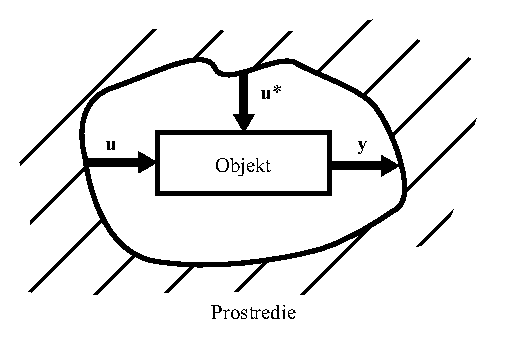
\includegraphics[width=80mm]{obr/OBRAZOK1_1.eps}
\caption{Stručný popis obrázku.}\label{OBRAZOK 1.1}
\end{figure}
%************ KONIEC **************
Nezabudnime, že popis obrázku je ukončený bodkou.

Na začiatku vety vypýšeme slovo Obrázok, kým všade inde používame skratku Obr.

\subsection{Formát obrázkov}

Pre ukladanie a zobrazenie obrázkov používame nasledovné súborové formáty:
\begin{itemize}
\item *.eps pre vektorovú grafiku (grafy, ilustrácie, priebehy)
\item *.png na screenshoty a
\item *.jpg na rasterovú grafiku (fotografie).
\end{itemize}

\subsection{Obrázky z Matlabu}

Z Matlabu exportujeme obrázky do formátu *.eps.

\section{Odvolávky na časti práce}
\label{hrusky}

Kapitolu, podkapitolu alebo podobné veci označíme príkazom "label", a nasledovne na nich odvoláme príkazom "ref". Napríklad v Kap. \ref{jablka} sme odvodili\ldots.
Na začiatku vety vypýšeme slovo Kapitola, kým všade inde používame skratku Kap. Podkapitoly a pod-podkapitoly v odvolávkach nerozlišujeme, na štruktúru dokumentu používame vždy Kap.

\section{Matematika}

Vzorce môžeme podľa potreby priamo písať do textu, napríklad: Číselná postupnosť - množina čísel $\vec{R} \{a_m, a_{m+1}, ...\}
= \{a_m\}_{m = n}^\infty$, respektíve to očíslovať a písať do samostatného riadku napríklad pomocou
  \begin{align}
  \label{mojarovnica}
    E_0 &= mc^2                              \\
    E &= \frac{mc^2}{\sqrt{1-\frac{v^2}{c^2}}}
  \end{align}
kde potom môžeme odvolávať na rovnicu pomocou Rov. \eqref{mojarovnica}. Pozor na to, že odkaz na čísla rovnice je zahrnutá v zátvorkách, to platí iba na rovnice, nie pre obrázky, tabuľky a štruktúru dokumentu. Namiesto príkazu align, môžeme používať aj eqnarray.

Na začiatku vety vypýšeme slovo Rovnica, kým všade inde používame skratku Rov.

\section{Programy, a užívateľské rozhrania}



\subsection{Programy}

Ak chceme písať názvy funkcií respektíve krátke časti počítačového kódu, môžeme na to používať príkaz \code{code}, napríklad \code{mojafunkcia()}.

Počítačový program môžeme jednoducho vložiť do textu pomocou
\lstset{language=exMatlab}
\begin{lstlisting}
N=1024;              % Pocet vzoriek
f1=1;                % Frekvencia harmonickeho signalu
FS=200;              % Frekvencia vzorkovania
n=0:N-1;             % Poradove cisla vzorky
x=sin(2*pi*f1*n/FS); % Generujeme signal, x(n)
[Rxx,Tau]=xcorr(x);  % Odhad autokorelacnej funkcie
\end{lstlisting}
Jazyk programu vieme určiť my, napríklad \code{Matlab} tu je rozšírený o extra príkazy.

\subsection{Užívateľské rozhrania}

Ak chceme označiť časti grafického rozhrania počítačového programu, cestu cez menu softvéru, názvy súborov atď, môžeme na to používať príkaz \code{gui}. Príkladom je \gui{File menu} alebo ikóna \gui{Môj počítač}.

\section{Tabuľky}


\begin{table}[htb]
\centering
\caption{Zoradenie metód na základe objemu apriórnych znalostí}
\begin{tabular}{ |l|c|c|c| }
  \hline
  \parbox[c]{3.5cm}{Metóda} & Kovariancia & \parbox[c]{3cm}{Hustota\\pravdepodobnosti}& Apriórna hustota\\ [0.2cm] \hline
  \parbox[c]{3.5cm}{Najmenšie štvorce} & Nie & Nie & Nie \\ [0.2cm] \hline
  \parbox[c]{3.5cm}{Najmenšie štvorce,\\Markov odhad}& Áno & Nie & Nie \\ [0.2cm]   \hline
  \parbox[c]{3.5cm}{Maximálna\\vierohodnosť}& Áno & Áno & Nie \\ [0.2cm] \hline
  \parbox[c]{3.5cm}{Bayesovské metódy} & Áno & Áno & Áno \\ [0.2cm] \hline
\end{tabular}
    \label{TABULKA_3_1}
\end{table}

Na tabuľky taktiež môžeme odvolávať pomocou Tab. \ref{TABULKA_3_1}. Tabuľky taktiež majú popis, dávame to nad tabuľkou.

Na začiatku vety vypíšeme slovo Tabuľka, kým všade inde používame skratku Tab.

\section{Fyzykálne jednotky}

Fyzikálne jednotky oddeľujeme medzerou od čísla a píšeme nezmeneným typom písma, t.j. nepoužívame šikmé písmo. Používame medzinárodne známe a akceptované jednotky a skratky jednotiek. Správne je teda 10 V, nesprávne je to 10V, 10 Volt, 10 \emph{V}.


\section{Bibliografické citácie}

Citovať môžeme nasledovne \cite{Eykhoff84}. Ak chceme citovať viacero autorov, tak môžeme to robiť naraz \cite{Fontes00,Eykhoff84}. Databazu citovaných dokumentov píšeme do súboru *.bib. Všetky typy dokumentov (kniha, článok etc.) má svoju vlastnú kategóriu. Autora publikácie môžeme aj napísať, napríklad že v práci Qin a Badgwell \cite{Qin99} dokázali že. Citácia je súčasťou vety, môžeme to kombinovať do vety \cite{Karny80} alebo dávať pred bodkou na koniec \cite{Far90}.

\section{Príklad}

Ak chceme uviesť inštrukčný príklad, potom na to máme prostredie
\begin{exmp}
Jožko má 5 melónov, vypočítajte hmotnosť Slnka.
\end{exmp}
kde príklad je ukončený znamienkom QED (štvorec).


\section{Záležitosti záverečnej práce}

\subsection{Obal}

Prvú stranu, takže obal a druhú (prázdnu stranu) nezviažeme do záverečnej práce, slúži to iba ako podklad na vyhotovenie obalu.

Na základe výnosu Ministerstva školstva Slovenskej republiky z 15. marca 2010 č. MŠSR-5/2010-071 ``o vzore obalu a titulného listu záverečnej, rigoróznej a habilitačnej práce a formáte výmeny údajov o záverečnej, rigoróznej a habilitačnej práci''  na obale záverečnej práce sa uvádzajú tieto informácie:
\begin{itemize}
\item  názov vysokej školy,
\item názov fakulty, ktorej je autor študentom, ak je zapísaný na štúdium študijného programu
uskutočňovaného na fakulte,
\item evidenčné číslo, ak bolo určené,
\item názov záverečnej práce, a ak sa použil, tak aj podnázov záverečnej práce,
\item meno, priezvisko, akademické tituly a vedecko-pedagogické tituly autora a
\item rok predloženia.
\end{itemize}

\subsection{Titulný list}

Na základe výnosu Ministerstva školstva Slovenskej republiky z 15. marca 2010 č. MŠSR-5/2010-071 ``o vzore obalu a titulného listu záverečnej, rigoróznej a habilitačnej práce a formáte výmeny údajov o záverečnej, rigoróznej a habilitačnej práci''  na titulnom liste záverečnej práce sa uvádzajú tieto informácie

\begin{itemize}
\item názov vysokej školy,
\item názov fakulty, ktorej je autor študentom, ak je zapísaný na štúdium študijného programu
uskutočňovaného na fakulte,
\item názov záverečnej práce, a ak sa použil, tak aj podnázov záverečnej práce,
\item označenie záverečnej práce: bakalárska práca, diplomová práca alebo dizertačná práca,
\item meno, priezvisko, akademické tituly a vedecko-pedagogické tituly autora,
\item názov študijného programu,
\item číslo a názov študijného odboru,
\item meno, priezvisko, akademické tituly a vedecko-pedagogické tituly školiteľa,
\item meno, priezvisko, akademické tituly a vedecko-pedagogické tituly konzultanta, ak bol pre
záverečnú prácu určený,
\item názov školiaceho pracoviska, ak pre záverečnú prácu bolo určené,
\item miesto a rok predloženia.
\end{itemize}


%Pisanie E, exponencia. nie e 

%\chapter{Ďalšie kapitoly}
\label{kap:3}
Každá kapitola začína na novej strane. Autor rieši zadanú problematiku. Na základe analýzy problému ponúka vlastné riešenia.

\section{Podkapitola}
\label{kap:1.1}

Podkapitoly záverečnej práce majú za úlohu členenie textu práce na dosiahnutie čo naj-väčšej prehľadnosti. Podkapitol môže byť viac, v ich názvoch sa používa desatinné číslovanie.

%[...]

%%%%%%% Koniec %%%%%%%%
\bibliographystyle{unsrt}
\addcontentsline{toc}{chapter}{Literat\'{u}ra}
\bibliography{bibliog}
\end{document}
